\documentclass[12pt]{article}

\usepackage[a4paper, top=2cm, bottom=2cm, left=2.5cm, right=2.5cm]{geometry}

\usepackage{amsmath, amssymb}
\usepackage{tikz}
\usetikzlibrary{arrows.meta,positioning,fit,calc}
\usepackage{multirow}
\usepackage{array}
\usepackage{siunitx}
\usepackage{enumitem}
\usepackage{float}
\usepackage{fontspec}
\usetikzlibrary{decorations.pathmorphing}
\usepackage{pdflscape}
\usepackage{tabularx}
\usepackage{booktabs}
\usepackage{graphicx}
\usepackage{listings}
\usepackage[table]{xcolor}
\usepackage{hyperref}
\usepackage{bookmark}
\usepackage{pdfpages}

% ---------------- FONTS ----------------
% Body font
\setmainfont[
    UprightFont = Handlee-Regular.ttf,
    AutoFakeBold = 2.5
]{Handlee}

% Heading font
\newfontfamily\headingfont{PT.ttf}

% verbatim font
\setmonofont{DejaVu Sans Mono} % or Noto Sans Mono

% ---------------- HANDWRITTEN MATH ----------------
\usepackage{mathastext}
\Mathastext
\everymath{\displaystyle}

% Optional spacing tweaks (more natural look)
% \setlength{\thinmuskip}{2mu}
% \setlength{\medmuskip}{2mu}

% ---------------- GENERAL ----------------
\setlength{\parindent}{0pt}
\pagenumbering{gobble}
\linespread{1.2}


\newcommand{\mychapter}[2]{%
    \phantomsection
    \hypertarget{#2}{}%
    \bookmark[level=0,dest=#2]{#1}%
    \begin{center}
        {\headingfont\Huge #1}
        \par
        \vspace{4pt}
        \hrule
    \end{center}
}

\newcommand{\mysection}[3]{%
    \phantomsection
    \hypertarget{#3}{}%
    \bookmark[level=1,dest=#3]{#1\space #2}%
    \noindent{\headingfont\Large #1\space #2\par}
    \vspace{4pt}
    \hrule
    \vspace{15pt}
}

\newcommand{\mysubsection}[2]{%
    \noindent{\headingfont\large #1\space #2\par}
    \vspace{4pt}
    \hrule
    \vspace{15pt}
}

\begin{document}
\vspace*{\fill}

\begin{figure}[H] % h = here, t = top, b = bottom, p = page of floats
    \centering
    \fbox{
\includegraphics[width=0.6\textwidth]{../2. Figures/cover.png}}
    \label{fig:myimage}
\end{figure}


\vspace{1cm}

\mychapter{Chapter 1 : Introduction \& Basic Concepts}{Chapter 1 : Introduction \& Basic Concepts}

This chapter introduces the fundamental concepts and vocabulary of thermodynamics needed for understanding energy and its transformations. It develops the basic ideas of systems, control volumes, properties, equilibrium, processes, and thermodynamic states. The chapter also establishes essential foundations involving dimensions, units, temperature, pressure, density, and specific properties. Together, these concepts provide the framework required for analyzing thermodynamic systems and solving engineering problems systematically.

\vspace*{\fill}

\newpage

\begin{center}
    {\headingfont\Huge Chapter Tree}
    \par
    \vspace{4pt}
    \hrule
\end{center}


\begin{verbatim}
│
├── 1–1 THERMODYNAMICS AND ENERGY
│   Introduces thermodynamics, energy, and fundamental energy principles.
│
├── 1–2 IMPORTANCE OF DIMENSIONS AND UNITS
│   Establishes dimensions, units, and commonly used measurement systems.
│
├── 1–3 SYSTEMS AND CONTROL VOLUMES
│   Defines systems, surroundings, boundaries, and control volumes.
│
├── 1–4 PROPERTIES OF A SYSTEM
│   Classifies system properties as intensive, extensive, and specific.
│
├── 1–5 DENSITY AND SPECIFIC GRAVITY
│   Defines density, specific volume, specific gravity, and specific weight.
│
├── 1–6 STATE AND EQUILIBRIUM
│   Describes thermodynamic states and different equilibrium conditions.
│
├── 1–7 PROCESSES AND CYCLES
│   Defines processes, process paths, quasi-equilibrium, and cycles.
│
├── 1–8 TEMPERATURE AND THE ZEROTH LAW OF THERMODYNAMICS
│   Introduces temperature measurement and the zeroth law.
│
├── 1–9 PRESSURE
│   Defines pressure and examines its variation within fluids.
│
├── 1–10 PRESSURE MEASUREMENT DEVICES
│   Introduces instruments used for measuring atmospheric and fluid pressures.
│
├── 1–11 PROBLEM-SOLVING TECHNIQUE
│    Presents a systematic approach for solving engineering problems.
│
└── A Remark on Significant Digits
    Explains appropriate precision and rounding of engineering results.
\end{verbatim}

\newpage


\mysection{1.1}{Thermodynamics and Energy}{1.1}

Thermodynamics is the science concerned with energy, energy transformations, and the interaction between energy and matter.

\mysubsection{}{Thermodynamics}

Energy may be viewed as the \textbf{ability to cause changes}.

The word thermodynamics originates from the Greek words \textit{therme} (heat) and \textit{dynamis} (power), reflecting the early development of the subject around converting heat into power.

Today, thermodynamics has a much broader scope and deals with:
\begin{itemize}
    \item Energy and its different forms.
    \item Energy transformations.
    \item Power generation.
    \item Refrigeration.
    \item Relationships among the properties of matter.
\end{itemize}

\mysubsection{}{Conservation of Energy}

The \textbf{conservation of energy principle} states that during an interaction, energy can change from one form to another, but the total amount of energy remains constant.

\begin{equation*}
\text{Energy cannot be created or destroyed; it can only change forms.}
\end{equation*}

For any system, the change in its energy content is equal to the difference between the energy entering and leaving the system.

\begin{equation*}
\Delta E = E_{\mathrm{in}}-E_{\mathrm{out}}
\end{equation*}

\textbf{\\ Example}

When a rock falls from a height, its potential energy is converted into kinetic energy. The total energy is conserved even though the form of energy changes.

\mysubsection{}{First and Second Laws of Thermodynamics}

The two fundamental laws of thermodynamics describe important characteristics of energy.

\begin{center}
    \begin{tabular}{|c|c|}
        \hline
        \textbf{Law} & \textbf{Main principle} \\
        \hline
        First law & Energy is conserved. \\
        \hline
        Second law & Energy has both quantity and quality. \\
        \hline
    \end{tabular}
\end{center}

The \textbf{first law of thermodynamics} is an expression of the conservation of energy principle and establishes energy as a thermodynamic property.

The \textbf{second law of thermodynamics} states that energy has quality as well as quantity. Actual processes occur in the direction of decreasing energy quality.

\textbf{\\ Example}

A hot cup of coffee placed in a cooler environment eventually loses heat and becomes cooler. However, a cool cup of coffee in the same environment does not spontaneously become hot.

Thus, energy naturally tends to be transferred from a region of higher temperature to a region of lower temperature, resulting in degradation of the usefulness or quality of energy.


\mysubsection{}{Macroscopic and Microscopic Approaches}

Matter consists of a very large number of particles called molecules. The properties observed at the macroscopic level arise from the behavior of these particles.

For example, the pressure of a gas results from momentum transfer between gas molecules and the walls of its container.

Two approaches can be used to study thermodynamics:

\begin{center}
    \begin{tabular}{|c|c|c|}
        \hline
        \textbf{Approach} & \textbf{Basis} & \textbf{Characteristic} \\
        \hline
        Classical thermodynamics &
        Macroscopic behavior &
        Direct and relatively simple \\
        \hline
        Statistical thermodynamics &
        Average microscopic behavior &
        More involved \\
        \hline
    \end{tabular}
\end{center}

\textbf{\\ Classical thermodynamics}

Classical thermodynamics does not require knowledge of the behavior of individual particles. It studies measurable macroscopic quantities and provides a direct and convenient method for solving engineering problems.

\textbf{\\ Statistical thermodynamics}

Statistical thermodynamics is based on the average behavior of large groups of individual particles. It is a microscopic approach and is more involved than classical thermodynamics.

In engineering applications, classical thermodynamics is generally the primary approach, while statistical thermodynamics may be used in a supporting role.

\mysubsection{}{Application Areas of Thermodynamics}

Interactions between energy and matter occur throughout nature. Consequently, thermodynamics is relevant to a wide range of engineering systems and everyday phenomena.

\begin{center}
    \begin{tabular}{|c|c|}
        \hline
        \textbf{Area} & \textbf{Examples} \\
        \hline
        Human body & Metabolic energy conversion and heat rejection \\
        \hline
        Household systems & Heating, air conditioning, refrigerators, water heaters \\
        \hline
        Appliances & Pressure cookers, irons, computers, televisions \\
        \hline
        Transportation & Automobile engines, aircraft, rockets, jet engines \\
        \hline
        Energy systems & Conventional and nuclear power plants, solar collectors \\
        \hline
        Industrial systems & Pumps, piping networks, and other thermal systems \\
        \hline
    \end{tabular}
\end{center}

\newpage




















\mysection{1.2}{Importance of Dimensions and Units}{1.2}

Any physical quantity can be characterized by its \textbf{dimensions}. The magnitudes assigned to dimensions are called \textbf{\\ units}. Some dimensions are selected as primary or fundamental dimensions, while others are expressed in terms of the primary dimensions and are called secondary or derived dimensions. :contentReference[oaicite:0]{index=0}

\mysubsection{}{Dimensions and Units}

\begin{center}
    \begin{tabular}{|c|c|c|}
        \hline
        \textbf{Quantity} & \textbf{Type} & \textbf{Description} \\
        \hline
        Mass, length, time, temperature & Primary dimensions & Fundamental dimensions \\
        \hline
        Velocity, energy, volume & Secondary dimensions & Expressed in terms of primary dimensions \\
        \hline
    \end{tabular}
\end{center}

Two unit systems are commonly used in engineering:
\begin{itemize}
    \item \textbf{SI system}: The metric International System of Units.
    \item \textbf{English system}: Also known as the United States Customary System (USCS).
\end{itemize}

The SI system has a simple decimal relationship between its units and is widely used in scientific and engineering work. The English system has less systematic relationships between units. Both systems are used in engineering, although SI units are emphasized. :contentReference[oaicite:1]{index=1} :contentReference[oaicite:2]{index=2}

\mysubsection{}{SI Fundamental Dimensions and Units}

The SI system is based on seven fundamental quantities and their corresponding units. :contentReference[oaicite:3]{index=3}

\begin{center}
    \begin{tabular}{|c|c|c|}
        \hline
        \textbf{Dimension} & \textbf{SI Unit} & \textbf{Symbol} \\
        \hline
        Length & meter & m \\
        \hline
        Mass & kilogram & kg \\
        \hline
        Time & second & s \\
        \hline
        Temperature & kelvin & K \\
        \hline
        Electric current & ampere & A \\
        \hline
        Amount of light & candela & cd \\
        \hline
        Amount of matter & mole & mol \\
        \hline
    \end{tabular}
\end{center}

The SI system uses standard prefixes to represent multiples and submultiples of units.
\begin{center}

\begin{tabular}{|c|c|c|}
    \hline
    \textbf{Multiple} & \textbf{Prefix} & \textbf{Symbol} \\
    \hline
    \(10^{24}\) & yotta & Y \\
    \hline
    \(10^{21}\) & zetta & Z \\
    \hline
    \(10^{18}\) & exa & E \\
    \hline
    \(10^{15}\) & peta & P \\
    \hline
    \(10^{12}\) & tera & T \\
    \hline
    \(10^{9}\) & giga & G \\
    \hline
    \(10^{6}\) & mega & M \\
    \hline
    \(10^{3}\) & kilo & k \\
    \hline
    \(10^{2}\) & hecto & h \\
    \hline
    \(10^{1}\) & deka & da \\
    \hline
\end{tabular}
\qquad
\begin{tabular}{|c|c|c|}
    \hline
    \textbf{Multiple} & \textbf{Prefix} & \textbf{Symbol} \\
    \hline
    \(10^{-1}\) & deci & d \\
    \hline
    \(10^{-2}\) & centi & c \\
    \hline
    \(10^{-3}\) & milli & m \\
    \hline
    \(10^{-6}\) & micro & \(\mu\) \\
    \hline
    \(10^{-9}\) & nano & n \\
    \hline
    \(10^{-12}\) & pico & p \\
    \hline
    \(10^{-15}\) & femto & f \\
    \hline
    \(10^{-18}\) & atto & a \\
    \hline
    \(10^{-21}\) & zepto & z \\
    \hline
    \(10^{-24}\) & yocto & y \\
    \hline
\end{tabular}

\end{center}

The SI prefixes are standard for all units and are widely used throughout engineering. :contentReference[oaicite:4]{index=4}

\mysubsection{}{Unit Conventions}

SI unit names are written without capitalization, even when derived from proper names. However, abbreviations of units derived from proper names are capitalized.

For example:
\begin{itemize}
    \item The SI unit is \textit{newton}, not \textit{Newton}.
    \item Its abbreviation is \(N\).
    \item A unit abbreviation is not pluralized.
    \item No period is used after a unit abbreviation unless it occurs at the end of a sentence.
\end{itemize}

Thus, \(5~m\) or \(5~\text{meters}\) is correct, while \(5~ms\) or \(5~\text{meter}\) is incorrect. :contentReference[oaicite:5]{index=5}
\begin{center}
    \begin{tabular}{|l|c|c|}
        \hline
        \textbf{Dimension} & \textbf{SI Unit} & \textbf{English Unit} \\
        \hline
        Length & \(1~\mathrm{m}\) & \(3.28084~\mathrm{ft}\) \\
        \hline
        Mass & \(1~\mathrm{kg}\) & \(2.20462~\mathrm{lbm}\) \\
        \hline
        Time & \(1~\mathrm{s}\) & \(1~\mathrm{s}\) \\
        \hline
        Force & \(1~\mathrm{N}\) & \(0.224809~\mathrm{lbf}\) \\
        \hline
        Pressure & \(1~\mathrm{kPa}\) & \(0.145038~\mathrm{psi}\) \\
        \hline
        Energy & \(1~\mathrm{kJ}\) & \(0.947817~\mathrm{Btu}\) \\
        \hline
        Power & \(1~\mathrm{kW}\) & \(1.34102~\mathrm{hp}\) \\
        \hline
        Volume & \(1~\mathrm{m^3}\) & \(35.3147~\mathrm{ft^3}\) \\
        \hline
        Specific Volume & \(1~\mathrm{m^3/kg}\) & \(16.0185~\mathrm{ft^3/lbm}\) \\
        \hline
        Density & \(1~\mathrm{kg/m^3}\) & \(0.062428~\mathrm{lbm/ft^3}\) \\
        \hline
        Specific Energy & \(1~\mathrm{kJ/kg}\) & \(0.429923~\mathrm{Btu/lbm}\) \\
        \hline
        Specific Weight & \(1~\mathrm{kN/m^3}\) & \(6.36588~\mathrm{lbf/ft^3}\) \\
        \hline
    \end{tabular}
\end{center}

\mysubsection{}{Dimensional Homogeneity}

An equation used in engineering must be \textbf{dimensionally homogeneous}. This means every term in an equation must have the same units.

If quantities with different units are added or subtracted, an error has occurred.

Dimensional analysis can therefore be used to:
\begin{itemize}
    \item Check the validity of equations.
    \item Detect errors in calculations.
    \item Verify that terms being added or subtracted have compatible dimensions.
\end{itemize}

A formula that is not dimensionally homogeneous is definitely incorrect. However, dimensional homogeneity alone does not guarantee that a formula is physically correct. :contentReference[oaicite:12]{index=12}

\textbf{\\ Example}

If an equation contains terms representing energy, every term added to or subtracted from those terms must also have units of energy.

\mysubsection{}{Unity Conversion Ratios}

Nonprimary dimensions can be formed from combinations of primary dimensions. Similarly, nonprimary units can be formed from combinations of primary units. :contentReference[oaicite:13]{index=13}

A \textbf{unity conversion ratio} is a ratio of two equivalent quantities and is exactly equal to one.

For example:

\begin{equation*}
\frac{1~\text{N}}{1~\text{kg}\cdot\text{m/s}^2}=1
\end{equation*}

and

\begin{equation*}
\frac{1~\text{lbf}}{32.174~\text{lbm}\cdot\text{ft/s}^2}=1
\end{equation*}

Since these ratios are equal to one, they can be inserted into calculations without changing the physical value of a quantity. They are used to convert units and maintain dimensional consistency. :contentReference[oaicite:14]{index=14}

\textbf{Important points:}
\begin{itemize}
    \item A unity conversion ratio is exactly equal to \(1\).
    \item Its inverse is also exactly equal to \(1\).
    \item The ratio should be arranged so that unwanted units cancel.
    \item Unity conversion ratios can be used to convert between different unit systems.
\end{itemize}

The use of unity conversion ratios is preferred over introducing the gravitational constant \(g_c\) merely to force units to match. :contentReference[oaicite:15]{index=15}

\newpage













\mysection{1.3}{Systems and Control Volumes}{1.3}

\mysubsection{}{System, Surroundings, and Boundary}

A \textbf{system} is defined as a quantity of matter or a region in space chosen for study.

The \textbf{surroundings} are the mass or region outside the system.

The \textbf{boundary} is the real or imaginary surface that separates the system from its surroundings.

\begin{center}
    \begin{tabular}{|c|c|}
        \hline
        \textbf{Term} & \textbf{Definition} \\
        \hline
        System & Quantity of matter or region in space chosen for study \\
        \hline
        Surroundings & Mass or region outside the system \\
        \hline
        Boundary & Surface separating the system from its surroundings \\
        \hline
    \end{tabular}
\end{center}

The boundary may be \textbf{fixed} or \textbf{movable}. It is the contact surface shared by the system and its surroundings.

Mathematically, the boundary has zero thickness. Therefore, it can neither contain mass nor occupy any volume.

\mysubsection{}{Types of Systems}

Systems are classified as \textbf{closed systems} or \textbf{open systems} depending on whether a fixed mass or a fixed region in space is selected for study.

\begin{center}
    \begin{tabular}{|c|c|c|}
        \hline
        \textbf{System} & \textbf{Mass Transfer} & \textbf{Energy Transfer} \\
        \hline
        Closed system & Not allowed & Allowed \\
        \hline
        Isolated system & Not allowed & Not allowed \\
        \hline
        Open system & Allowed & Allowed \\
        \hline
    \end{tabular}
\end{center}

\begin{figure}[H] % h = here, t = top, b = bottom, p = page of floats
    \centering
    \fbox{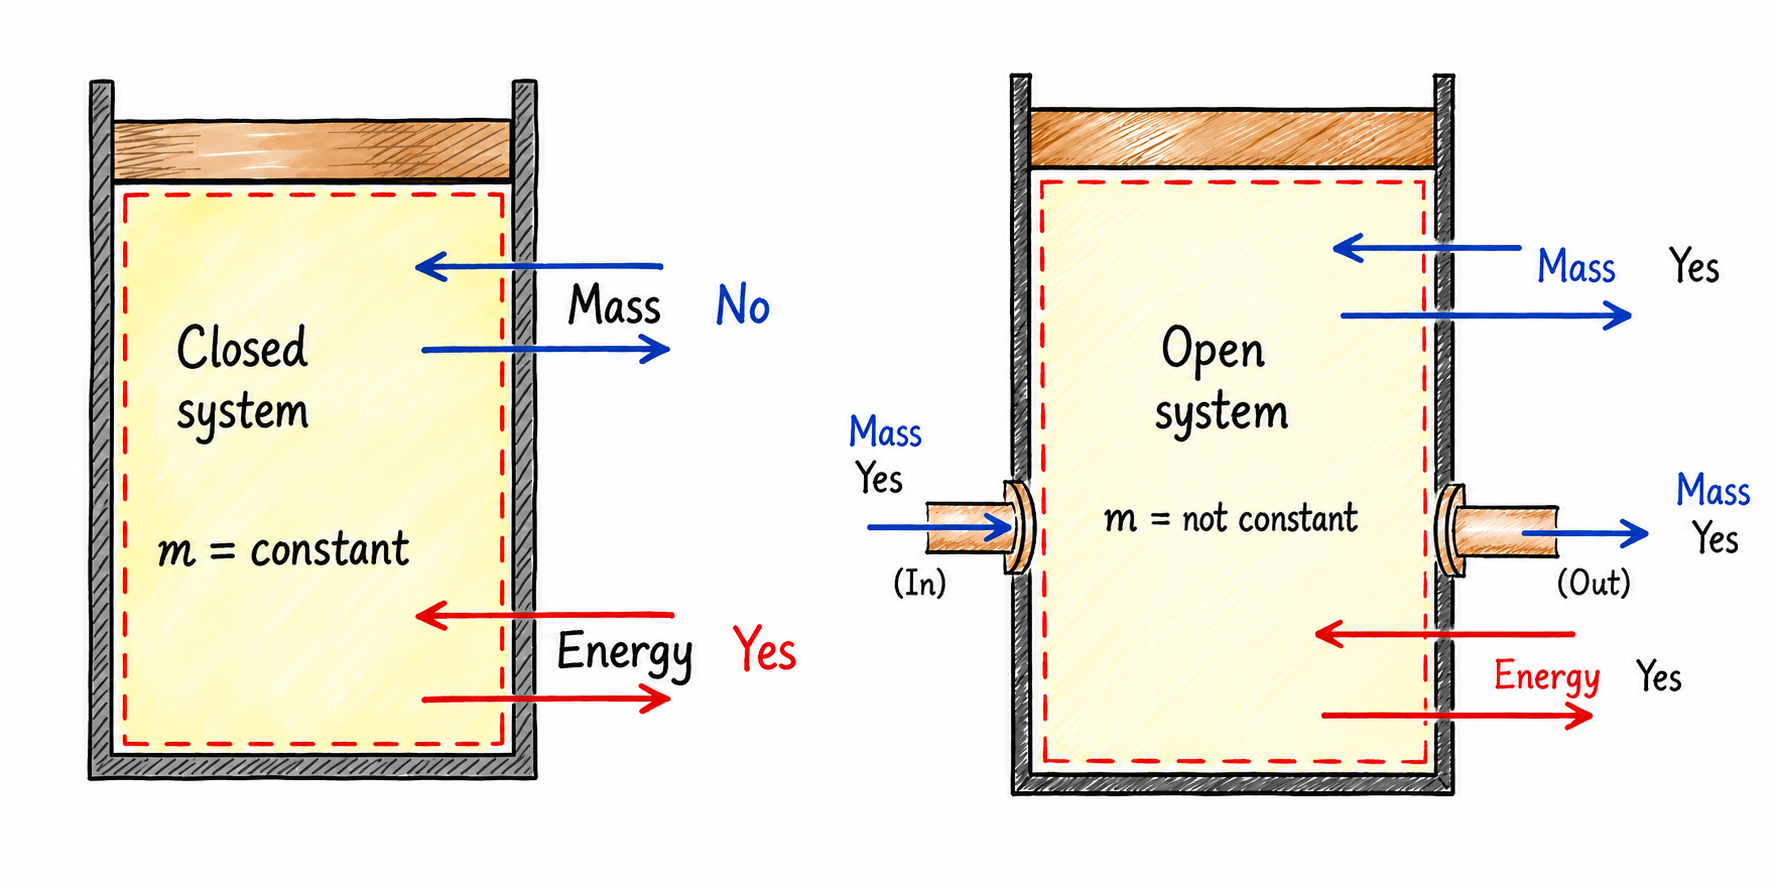
\includegraphics[width=0.65\textwidth]{../2. Figures/Figure : 1.png}}
    \label{fig:myimage}
    \caption{Types of System}
\end{figure}



\mysubsection{}{Closed System}

A \textbf{closed system}, also called a \textbf{control mass}, consists of a fixed amount of mass.

No mass can cross the boundary of a closed system, but energy in the form of heat or work can cross the boundary.

The volume of a closed system does not necessarily have to remain fixed.

\textbf{\\ Isolated System}

An \textbf{isolated system} is a special type of closed system in which neither mass nor energy is allowed to cross the boundary.

\begin{equation*}
m=\text{constant}
\end{equation*}


\mysubsection{}{Example of a Closed System}

Consider a piston-cylinder device containing gas.

If the gas is selected as the system, the inner surfaces of the piston and cylinder form the boundary.

Since no mass crosses this boundary, the gas forms a closed system.

Energy may cross the boundary, for example, when the gas is heated. The boundary may also move because the piston can move.

\begin{center}
    \begin{tabular}{|c|c|}
        \hline
        \textbf{Part} & \textbf{Description} \\
        \hline
        System & Gas enclosed in the cylinder \\
        \hline
        Boundary & Inner surfaces of piston and cylinder \\
        \hline
        Surroundings & Everything outside the gas \\
        \hline
        Mass transfer & None \\
        \hline
        Energy transfer & Possible \\
        \hline
        Boundary & May move with the piston \\
        \hline
    \end{tabular}
\end{center}

\mysubsection{}{Open System}

An \textbf{open system}, also called a \textbf{control volume}, is a properly selected region in space.

A control volume usually encloses a device through which mass flows, such as:
\begin{itemize}
    \item Compressor
    \item Turbine
    \item Nozzle
\end{itemize}

Both \textbf{mass} and \textbf{energy} can cross the boundary of a control volume.


A large number of engineering problems involve mass flow into and out of a system. Such systems are therefore more conveniently modeled as control volumes rather than control masses.

\mysubsection{}{Selection of a Control Volume}

In general, any arbitrary region in space can be selected as a control volume.

There are no strict rules for selecting a control volume. However, a proper choice can greatly simplify the analysis.

For example, when analyzing the flow of air through a nozzle, the region within the nozzle is a convenient choice for the control volume.

\textbf{Control Surface}

The boundary of a control volume is called a \textbf{control surface}.

A control surface may be:
\begin{itemize}
    \item Real.
    \item Imaginary.
    \item Fixed.
    \item Moving.
\end{itemize}

For a nozzle, the inner wall of the nozzle forms the real part of the control surface, while the entrance and exit areas form imaginary parts of the control surface.

\mysubsection{}{Fixed and Moving Control Volumes}

A control volume may be fixed in size and shape or may involve a moving boundary.

\begin{center}
    \begin{tabular}{|c|c|}
        \hline
        \textbf{Type} & \textbf{Description} \\
        \hline
        Fixed control volume & Size and shape remain constant \\
        \hline
        Moving control volume & Boundary can move \\
        \hline
        Real boundary & Corresponds to a physical surface \\
        \hline
        Imaginary boundary & Used where no physical surface exists \\
        \hline
    \end{tabular}
\end{center}

Most control volumes have fixed boundaries and therefore do not involve moving boundaries.

A control volume can involve heat and work interactions in addition to mass interaction.

\mysubsection{}{Example of an Open System}

Consider a water heater in which cold water enters the tank and hot water leaves the tank.

Since hot water continuously leaves the tank and is replaced by cold water, it is not convenient to choose a fixed mass as the system.

Instead, the region enclosed by the interior surfaces of the tank can be selected as the control volume.

The cold water entering the tank and the hot water leaving the tank represent mass crossing the control surface.

\begin{center}
    \begin{tabular}{|c|c|}
        \hline
        \textbf{Part} & \textbf{Description} \\
        \hline
        Control volume & Interior region of the water heater \\
        \hline
        Control surface & Interior surfaces of the tank \\
        \hline
        Mass entering & Cold water \\
        \hline
        Mass leaving & Hot water \\
        \hline
        Energy interaction & Heat transferred to the water \\
        \hline
    \end{tabular}
\end{center}

The water heater therefore provides an example of an open system with mass entering and leaving the control volume.

\newpage
\mysubsection{}{Importance of Proper System Selection}

The system under study must be defined carefully in an engineering analysis.

In simple problems, the system may be obvious and its definition may appear unnecessary. In more complicated problems, however, selecting an appropriate system can greatly simplify the analysis.

\textbf{Closed System vs Control Volume}

\begin{center}
    \begin{tabular}{|c|c|c|}
        \hline
        \textbf{Feature} & \textbf{Closed System} & \textbf{Control Volume} \\
        \hline
        Amount of matter & Fixed & May change \\
        \hline
        Mass crossing boundary & No & Yes \\
        \hline
        Energy crossing boundary & Yes & Yes \\
        \hline
        Boundary & Real or imaginary & Real or imaginary \\
        \hline
        Boundary motion & May be fixed or movable & May be fixed or movable \\
        \hline
        Typical example & Piston-cylinder & Turbine or nozzle \\
        \hline
    \end{tabular}
\end{center}


\newpage












\mysection{1.4}{Properties of a System}{1.4}

\mysubsection{}{Properties of a System}

Any characteristic of a system is called a \textbf{property}. Common thermodynamic properties include pressure $P$, temperature $T$, volume $V$, and mass $m$. Other properties include viscosity, thermal conductivity, modulus of elasticity, thermal expansion coefficient, electrical resistivity, velocity, and elevation.

Properties are classified as \textbf{intensive} or \textbf{extensive} depending on whether they depend on the amount of matter present in the system.

\textbf{\\ Intensive Properties}
    
Intensive properties are independent of the mass or size of the system.

Examples:
\begin{center}
    \begin{tabular}{|c|c|}
        \hline
        \textbf{Property} & \textbf{Examples} \\
        \hline
        Intensive & Temperature, pressure, density \\
        \hline
    \end{tabular}
\end{center}

\textbf{\\ Extensive Properties}

Extensive properties depend on the size or amount of matter in the system.

Examples:
\begin{center}
    \begin{tabular}{|c|c|}
        \hline
        \textbf{Property} & \textbf{Examples} \\
        \hline
        Extensive & Mass, volume, total momentum \\
        \hline
    \end{tabular}
\end{center}

\textbf{\\ Identifying Intensive and Extensive Properties}

An easy criterion is to imagine dividing the system into two equal parts:
\begin{center}
    \begin{tabular}{|c|c|}
        \hline
        \textbf{Property type} & \textbf{Effect of division} \\
        \hline
        Intensive & Value remains unchanged \\
        \hline
        Extensive & Value becomes proportional to the amount of matter \\
        \hline
    \end{tabular}
\end{center}


\begin{figure}[H] % h = here, t = top, b = bottom, p = page of floats
    \centering
    \fbox{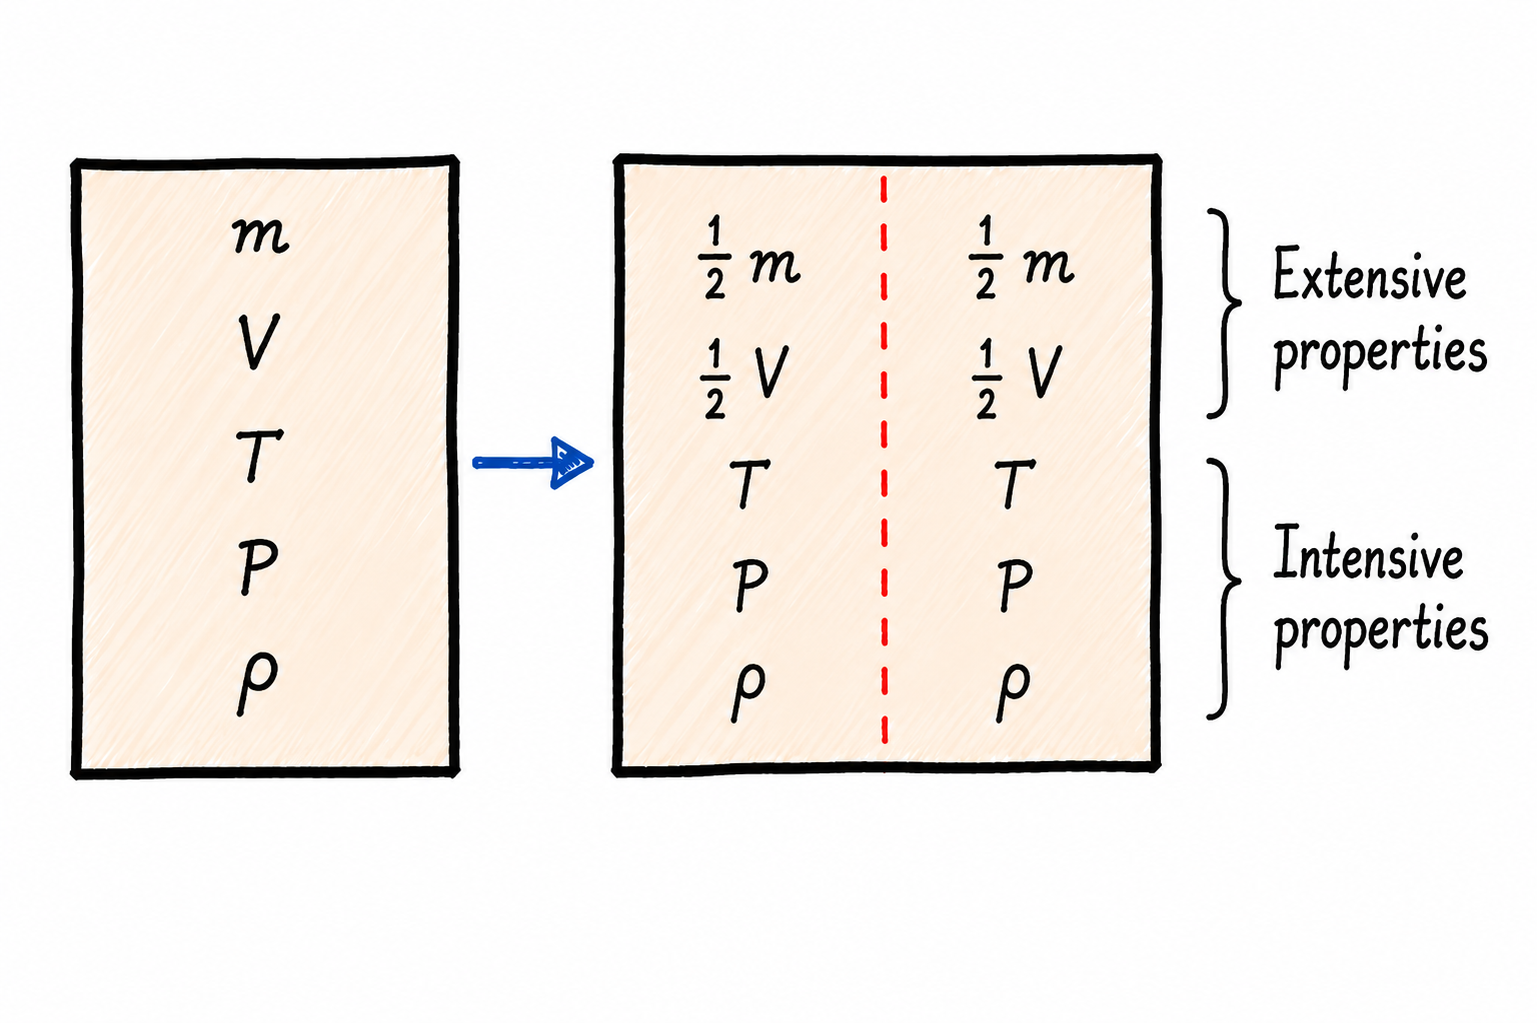
\includegraphics[width=0.5\textwidth]{../2. Figures/Figure : 2.png}}
    \label{fig:myimage}
    \caption{Test to identify type of property}
\end{figure}


\mysubsection{}{Specific Properties}

An extensive property expressed per unit mass is called a \textbf{specific property}.

Specific properties are intensive because dividing an extensive property by mass removes its dependence on the size of the system.

For specific volume,
\begin{equation*}
    v = \frac{V}{m}
\end{equation*}

where:
\begin{itemize}
    \item $v$ = specific volume
    \item $V$ = total volume
    \item $m$ = mass
\end{itemize}

Specific total energy is another example:
\begin{equation*}
    e = \frac{E}{m}
\end{equation*}

where $E$ is the total energy of the system.

\mysubsection{}{Continuum}

Matter is actually composed of discrete atoms and molecules. In thermodynamic analysis, however, it is usually convenient to ignore the molecular structure and regard matter as a continuous, homogeneous substance called a \textbf{continuum}.

The continuum idealization allows:
\begin{itemize}
    \item properties to be treated as point functions,
    \item properties to vary continuously throughout the system, and
    \item abrupt molecular-scale variations to be neglected.
\end{itemize}

The continuum assumption is valid when the characteristic dimension of the system is much larger than the distance between molecules or, more specifically, the mean free path of the molecules.

For oxygen at $1$ atm and $20^\circ\mathrm{C}$:
\begin{equation*}
    d_{\mathrm{O_2}} \approx 3 \times 10^{-10}\,\mathrm{m}
\end{equation*}

\begin{equation*}
    \lambda \approx 6.3 \times 10^{-8}\,\mathrm{m}
\end{equation*}

where $\lambda$ is the mean free path. Even in a volume of $1\,\mathrm{mm^3}$, there are approximately
\begin{equation*}
    3 \times 10^{16}
\end{equation*}
molecules of oxygen under these conditions.

Thus, for ordinary engineering systems, the molecular structure can usually be ignored and the substance can be treated as a continuum.

At very high vacuum or at very high elevations, the mean free path becomes large relative to the characteristic dimension of the system. In such cases, the continuum approximation may fail and rarefied-gas-flow theory must be used.








\newpage

\mysection{1.5}{Density \& Specific Gravity}{1.5}

\mysubsection{}{Density}

Density is defined as the mass per unit volume of a substance.

\begin{equation*}
    \rho = \frac{m}{V}
\end{equation*}

where $\rho$ is density, $m$ is mass, and $V$ is volume.

The SI unit of density is $\mathrm{kg/m^3}$.

For a differential volume element, density can also be expressed as

\begin{equation*}
    \rho = \frac{\delta m}{\delta V}
\end{equation*}

The density of a substance generally depends on temperature and pressure. For most gases, density is approximately proportional to pressure and inversely proportional to temperature.

Liquids and solids are essentially incompressible, so their density changes only slightly with pressure. Their density is generally more sensitive to temperature than to pressure.

\mysubsection{}{Specific Volume}

Specific volume is defined as the volume occupied per unit mass. It is the reciprocal of density.

\begin{equation*}
    v = \frac{V}{m} = \frac{1}{\rho}
\end{equation*}

The SI unit of specific volume is $\mathrm{m^3/kg}$.

Thus,

\begin{equation*}
    \rho v = 1
\end{equation*}

\textbf{\\ Density--Specific Volume Relationship}

\begin{center}
    \begin{tabular}{|c|c|c|}
        \hline
        \textbf{Quantity} & \textbf{Definition} & \textbf{SI Unit} \\
        \hline
        Density, $\rho$ & $\dfrac{m}{V}$ & $\mathrm{kg/m^3}$ \\
        \hline
        Specific volume, $v$ & $\dfrac{V}{m}$ & $\mathrm{m^3/kg}$ \\
        \hline
    \end{tabular}
\end{center}

\mysubsection{}{Specific Gravity}

Specific gravity, also called relative density, is the ratio of the density of a substance to the density of a standard substance at a specified temperature.

For most applications in this section, water at $4^\circ\mathrm{C}$ is used as the standard, with

\begin{equation*}
    \rho_{\mathrm{H_2O}} = 1000\ \mathrm{kg/m^3}
\end{equation*}

The specific gravity is therefore

\begin{equation*}
    SG = \frac{\rho}{\rho_{\mathrm{H_2O}}}
\end{equation*}

Specific gravity is \textbf{dimensionless} because it is a ratio of two densities having the same units.

\textbf{\\ Interpretation of Specific Gravity}

\begin{center}
    \begin{tabular}{|c|c|}
        \hline
        \textbf{Specific Gravity} & \textbf{Interpretation} \\
        \hline
        $SG < 1$ & Substance is less dense than water \\
        \hline
        $SG = 1$ & Density is equal to that of water \\
        \hline
        $SG > 1$ & Substance is denser than water \\
        \hline
    \end{tabular}
\end{center}

For example, mercury has a specific gravity of $13.6$ at $0^\circ\mathrm{C}$. Hence,

\begin{equation*}
    \rho_{\mathrm{Hg}} = 13.6(1000)
    = 13600\ \mathrm{kg/m^3}
\end{equation*}

In SI units, the numerical value of specific gravity is also equal to the numerical value of density when density is expressed in $\mathrm{g/cm^3}$ or $\mathrm{kg/L}$.

Since

\begin{equation*}
    1\ \mathrm{g/cm^3} = 1\ \mathrm{kg/L}
    = 1000\ \mathrm{kg/m^3}
\end{equation*}

a substance with $SG=13.6$ has a density of $13.6\ \mathrm{g/cm^3}$ or $13.6\ \mathrm{kg/L}$.

\mysubsection{}{Specific Weight}

Specific weight is defined as the weight of a substance per unit volume.

\begin{equation*}
    \gamma_s = \rho g
\end{equation*}

where $\gamma_s$ is the specific weight, $\rho$ is the density, and $g$ is the gravitational acceleration.

The SI unit of specific weight is $\mathrm{N/m^3}$.
\newpage
























\mysection{1.6}{State and Equilibrium}{1.6}

\mysubsection{}{State of a System}

The \textbf{state} of a system is the condition of the system described by the values of its properties. When a system is not undergoing any change, its properties can be measured or calculated throughout the system, providing a complete description of its state.

At a given state, all the properties of the system have fixed values. If the value of even one property changes, the system changes to a different state.

\textbf{\\ Equilibrium}

Thermodynamics deals primarily with \textbf{equilibrium states}. Equilibrium implies a state of balance in which there are no unbalanced potentials or driving forces within the system.

A system in equilibrium does not undergo any change when it is isolated from its surroundings.

A system is in \textbf{thermodynamic equilibrium} only when all the relevant types of equilibrium are satisfied.

\mysubsection{}{Types of Equilibrium}


\begin{center}
    \begin{tabular}{|c|c|}
        \hline
        \textbf{Type} & \textbf{Condition} \\
        \hline
        Thermal equilibrium & No temperature difference within the system \\
        \hline
        Mechanical equilibrium & No pressure changes with time at any point \\
        \hline
        Phase equilibrium & Mass of each phase remains at an equilibrium level \\
        \hline
        Chemical equilibrium & Chemical composition does not change with time \\
        \hline
    \end{tabular}
\end{center}

\textbf{\\ Condition for Thermodynamic Equilibrium}

A system cannot be considered to be in thermodynamic equilibrium unless all the relevant equilibrium requirements are simultaneously satisfied.

\mysubsection{}{The State Postulate}

Although the state of a system is described by its properties, it is not necessary to specify all the properties to completely fix the state. Once a sufficient number of independent properties are specified, the remaining properties automatically assume definite values.

\textbf{\\ State Postulate}

The state of a simple compressible system is completely specified by \textbf{two independent, intensive properties}.

\textbf{\\ Simple Compressible System}

A simple compressible system is a system in which electrical, magnetic, gravitational, motion, and surface-tension effects are absent or negligible.

These effects are generally negligible in most engineering problems. If any such effect is significant, an additional property must be specified for each important effect.

For example, if gravitational effects are significant, the elevation $z$ must be specified in addition to the two properties required by the state postulate.

\textbf{\\ Independent Properties}

The two properties used to specify the state must be \textbf{independent}.

Two properties are independent if one property can be varied while the other is held constant.

Temperature and specific volume are always independent properties. Therefore, for a simple compressible system,

\begin{equation*}
    T \text{ and } v
\end{equation*}

can be used together to completely specify the state.

Temperature and pressure behave differently depending on the phase condition. For a single-phase system, $T$ and $P$ are independent properties.

For a multiphase system, however, temperature and pressure can become dependent properties. During a phase-change process,

\begin{equation*}
    T = f(P)
\end{equation*}

Thus, temperature and pressure alone are not sufficient to fix the state of a two-phase system.

\textbf{\\ Example of State Specification}

For nitrogen, two independent intensive properties such as temperature and specific volume can completely specify the state:

\begin{equation*}
    T = 25^\circ\mathrm{C}
\end{equation*}

\begin{equation*}
    v = 0.9\ \mathrm{m^3/kg}
\end{equation*}

Hence, no additional independent intensive property is required for a simple compressible nitrogen system under the assumptions of the state postulate.

\newpage














\mysection{1.7}{Processes and Cycles}{1.7}

\mysubsection{}{Process}

Any change that a system undergoes from one equilibrium state to another is called a \textbf{process}.

The series of equilibrium states through which the system passes during a process is called the \textbf{path of the process}.

A process is completely described by specifying:
\begin{itemize}
    \item the initial state,
    \item the final state,
    \item the path followed by the system, and
    \item the interactions between the system and its surroundings.
\end{itemize}

\textbf{\\ Quasi-Equilibrium Process}

A process during which the system remains infinitesimally close to an equilibrium state at all times is called a \textbf{quasi-equilibrium} or \textbf{quasi-static process}.

It can be viewed as a sufficiently slow process that allows the system to adjust internally so that the properties remain nearly uniform throughout the system.

\textbf{\\ Example : }

Consider a gas in a piston-cylinder device.

During a \textbf{very rapid compression}, the molecules near the piston do not have sufficient time to redistribute. A high-pressure region develops near the piston, and the system is not in equilibrium.

During a \textbf{slow compression}, the molecules have enough time to redistribute. The pressure remains nearly uniform throughout the cylinder, so the process can be treated as quasi-equilibrium.

\textbf{\\ Importance of Quasi-Equilibrium Processes}

A quasi-equilibrium process is an idealization rather than an exact representation of a real process. However, many actual processes can be approximated by quasi-equilibrium processes with negligible error.

Engineers are interested in quasi-equilibrium processes because:
\begin{itemize}
    \item they are easier to analyze, and
    \item work-producing devices deliver the most work when operating through quasi-equilibrium processes.
\end{itemize}

Therefore, quasi-equilibrium processes provide useful standards against which actual processes can be compared.

\mysubsection{}{Process Diagrams and Process Path}

Thermodynamic processes can be represented graphically by using thermodynamic properties as coordinates.

Common properties used as coordinates are:
\begin{center}
    \begin{tabular}{|c|c|}
        \hline
        \textbf{Coordinate} & \textbf{Property} \\
        \hline
        $T$ & Temperature \\
        \hline
        $P$ & Pressure \\
        \hline
        $V$ or $v$ & Volume or specific volume \\
        \hline
    \end{tabular}
\end{center}

For example, a compression process can be represented on a $P$-$V$ diagram, with the process path connecting the initial and final states.

The process path has physical significance for a \textbf{quasi-equilibrium process} because every point on the path represents an equilibrium state.

For a \textbf{nonquasi-equilibrium process}, the entire system cannot be described by a single equilibrium state at each instant. Therefore, a process path for the system as a whole cannot be defined. Such a process is represented by a dashed line between the initial and final states.

\mysubsection{}{Common Types of Processes}

The prefix \textbf{iso-} indicates that a particular property remains constant during a process.

\textbf{\\ Isothermal Process}

An isothermal process is a process during which the temperature remains constant.

\begin{equation*}
    T = \text{constant}
\end{equation*}

\textbf{\\ Isobaric Process}

An isobaric process is a process during which the pressure remains constant.

\begin{equation*}
    P = \text{constant}
\end{equation*}

\textbf{\\ Isochoric Process}

An isochoric process, also called an isometric process, is a process during which the specific volume remains constant.

\begin{equation*}
    v = \text{constant}
\end{equation*}

\mysubsection{}{Cycle}

A system is said to undergo a \textbf{cycle} if it returns to its initial state at the end of the process.

Thus, for a cycle,

\begin{equation*}
    \text{Initial state} = \text{Final state}
\end{equation*}

Although the system may undergo several processes while completing a cycle, the final state is identical to the initial state.

\begin{figure}[H] % h = here, t = top, b = bottom, p = page of floats
    \centering
    \fbox{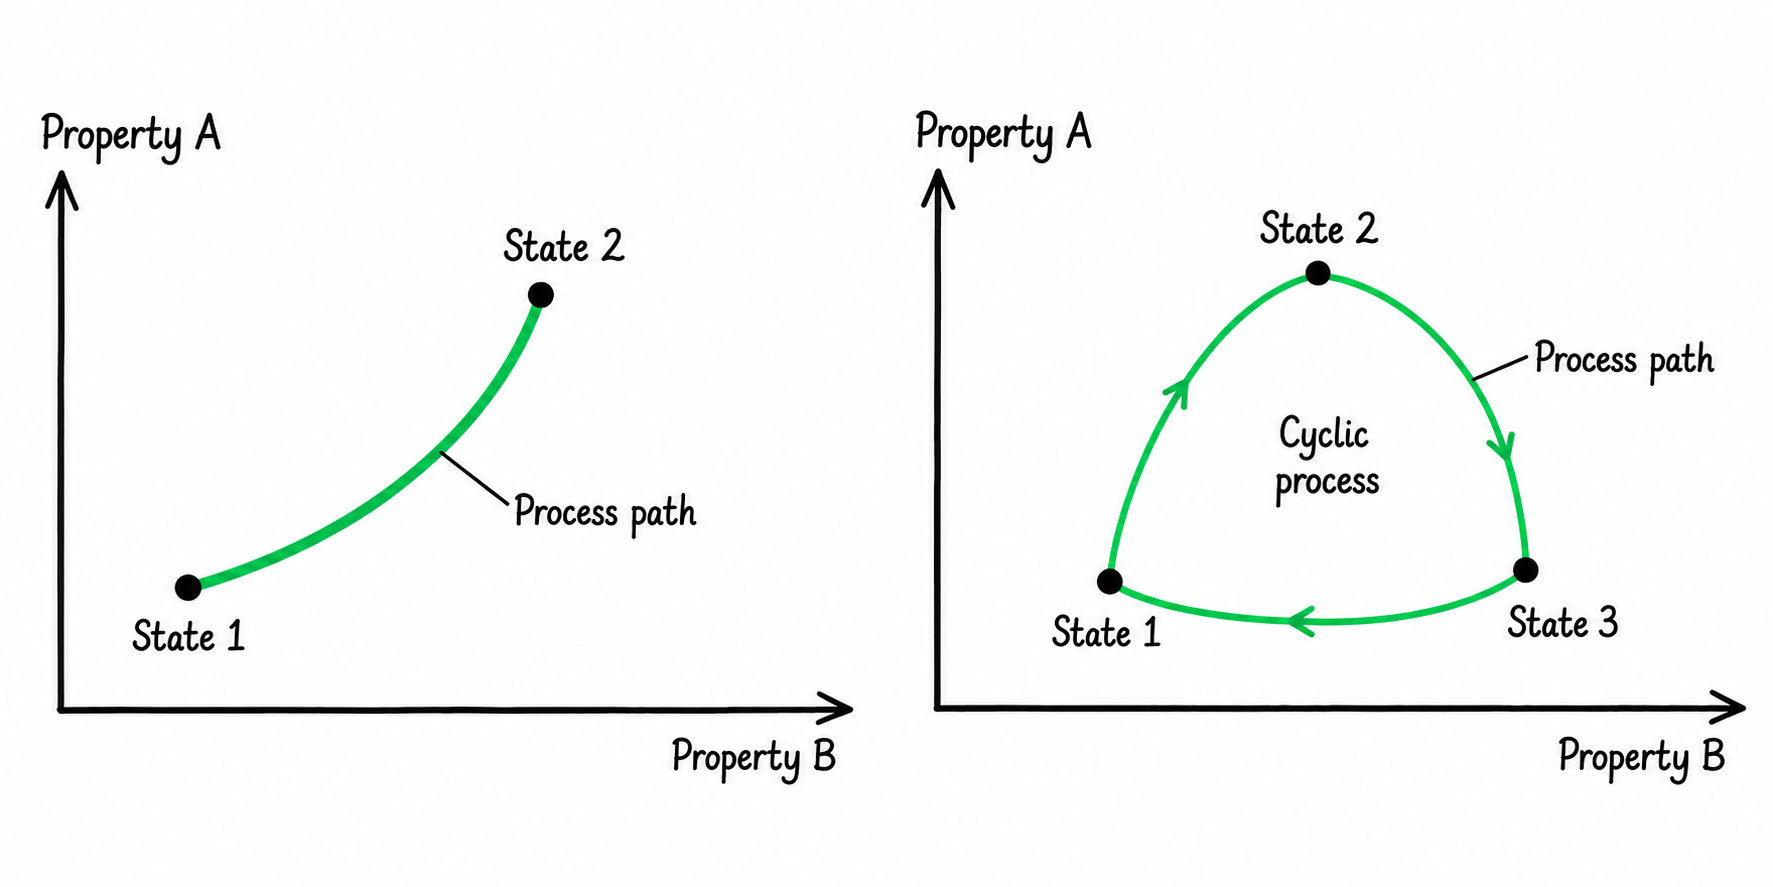
\includegraphics[width=0.55\textwidth]{../2. Figures/Figure : 3.png}}
    \label{fig:myimage}
    \caption{Process \& Cycle}
\end{figure}

\mysubsection{}{Steady-Flow Process}

\begin{center}
    \begin{tabular}{|c|c|}
        \hline
        \textbf{Term} & \textbf{Meaning} \\
        \hline
        Steady & No change with time \\
        \hline
        Uniform & No change with location \\
        \hline
    \end{tabular}
\end{center}

A large number of engineering devices operate for long periods under essentially constant conditions and can be modeled as \textbf{steady-flow devices}.

A \textbf{steady-flow process} is a process in which fluid flows through a control volume steadily.

During a steady-flow process:
\begin{itemize}
    \item fluid properties may vary from point to point within the control volume,
    \item at any fixed point, the fluid properties do not change with time,
    \item the volume of the control volume remains constant,
    \item the mass contained in the control volume remains constant, and
    \item the total energy content of the control volume remains constant.
\end{itemize}

Thus,

\begin{equation*}
    V = \text{constant}
\end{equation*}

\begin{equation*}
    m = \text{constant}
\end{equation*}

\begin{equation*}
    E = \text{constant}
\end{equation*}

Steady-flow conditions can be closely approximated in devices intended for continuous operation, such as turbines, pumps, and boilers.

\newpage

















\mysection{1.8}{Temperature and the Zeroth Law of Thermodynamics}{1.8}

\mysubsection{}{Temperature}

Temperature is a measure of the thermal state of a substance and is commonly associated with the degree of hotness or coldness. Human senses provide only a qualitative indication of temperature and cannot be relied upon for accurate measurement.

Accurate temperature measurement is possible because certain properties of materials change with temperature in a repeatable and predictable manner. For example, a mercury-in-glass thermometer operates on the expansion of mercury with temperature.

\textbf{\\ Thermal Equilibrium}

When two bodies at different temperatures are brought into contact, heat is transferred from the body at higher temperature to the body at lower temperature.

This transfer continues until both bodies reach the same temperature. At that point, heat transfer stops and the bodies are said to be in \textbf{thermal equilibrium}.

The only requirement for thermal equilibrium is equality of temperature.

\mysubsection{}{Zeroth Law of Thermodynamics}

The \textbf{zeroth law of thermodynamics} states:

\textbf{\\ Zeroth Law}

If two bodies are each in thermal equilibrium with a third body, then they are in thermal equilibrium with each other.

The zeroth law provides the basis for temperature measurement. A thermometer can be regarded as the third body. If two bodies produce the same temperature reading on the thermometer, they are in thermal equilibrium with each other even when they are not in direct contact.

\textbf{\\ Temperature Measurement}

The zeroth law establishes temperature as a property that can be compared between systems.

Thus, a thermometer can be used to determine whether two bodies are at the same temperature without requiring them to be in direct contact.

\mysubsection{}{Temperature Scales}

Temperature scales provide a common basis for assigning numerical values to temperature.

They are based on reproducible reference states. Two historically important reference states are:

\begin{center}
    \begin{tabular}{|c|c|}
        \hline
        \textbf{Reference state} & \textbf{Description} \\
        \hline
        Ice point & Ice and water in equilibrium at $1$ atm \\
        \hline
        Steam point & Liquid water and water vapor in equilibrium at $1$ atm \\
        \hline
    \end{tabular}
\end{center}


\textbf{\\ Temperature Scales Comparison}

\begin{center}
    \begin{tabular}{|c|c|c|}
        \hline
        \textbf{Scale} & \textbf{Ice Point} & \textbf{Steam Point} \\
        \hline
        Celsius & $0^\circ\mathrm{C}$ & $100^\circ\mathrm{C}$ \\
        \hline
        Fahrenheit & $32^\circ\mathrm{F}$ & $212^\circ\mathrm{F}$ \\
        \hline
    \end{tabular}
\end{center}

\mysubsection{}{Thermodynamic Temperature Scales}

A thermodynamic temperature scale should be independent of the properties of any particular substance.

The thermodynamic temperature scale in the SI system is the \textbf{Kelvin scale}, while the corresponding scale in the English system is the \textbf{Rankine scale}.

\textbf{\\ Kelvin Scale}

The thermodynamic temperature unit in the SI system is the \textbf{kelvin}, symbol $K$.

The degree symbol is not used with kelvin. Thus, the correct notation is $300\ K$, not $300^\circ K$.

The lowest possible temperature is \textbf{absolute zero}:

\begin{equation*}
    T = 0\ K
\end{equation*}

Absolute zero corresponds to

\begin{equation*}
    T = -273.15^\circ\mathrm{C}
\end{equation*}

\textbf{\\ Rankine Scale}

The thermodynamic temperature scale in the English system is the \textbf{Rankine scale}.

Its temperature unit is the \textbf{rankine}, symbol $R$.

\mysubsection{}{Ideal-Gas Temperature Scale}

An ideal-gas temperature scale is nearly identical to the Kelvin scale.

It can be measured using a constant-volume gas thermometer, which consists of a rigid vessel containing a gas at low pressure.

At sufficiently low pressure and constant volume, the temperature of the gas is proportional to its pressure.

The relationship can be expressed as

\begin{equation*}
    T = a + bP
\end{equation*}

where $a$ and $b$ are experimentally determined constants.

The constants are determined by measuring the gas pressure at two reproducible reference temperatures.

If the ice point is assigned $0^\circ\mathrm{C}$ and the steam point is assigned $100^\circ\mathrm{C}$, the resulting gas-temperature scale agrees with the Celsius scale.

On extrapolation to zero pressure, the temperature is

\begin{equation*}
    T = -273.15^\circ\mathrm{C}
\end{equation*}

This corresponds to absolute zero.

By assigning zero temperature at zero absolute pressure, the relation becomes

\begin{equation*}
    T = bP
\end{equation*}

This provides an absolute gas-temperature scale.

The absolute gas-temperature scale agrees with the thermodynamic temperature scale over the range in which the gas thermometer can be used, although it cannot be used at extremely low or extremely high temperatures because of phenomena such as condensation, dissociation, and ionization.

\begin{figure}[H] % h = here, t = top, b = bottom, p = page of floats
    \centering
    \fbox{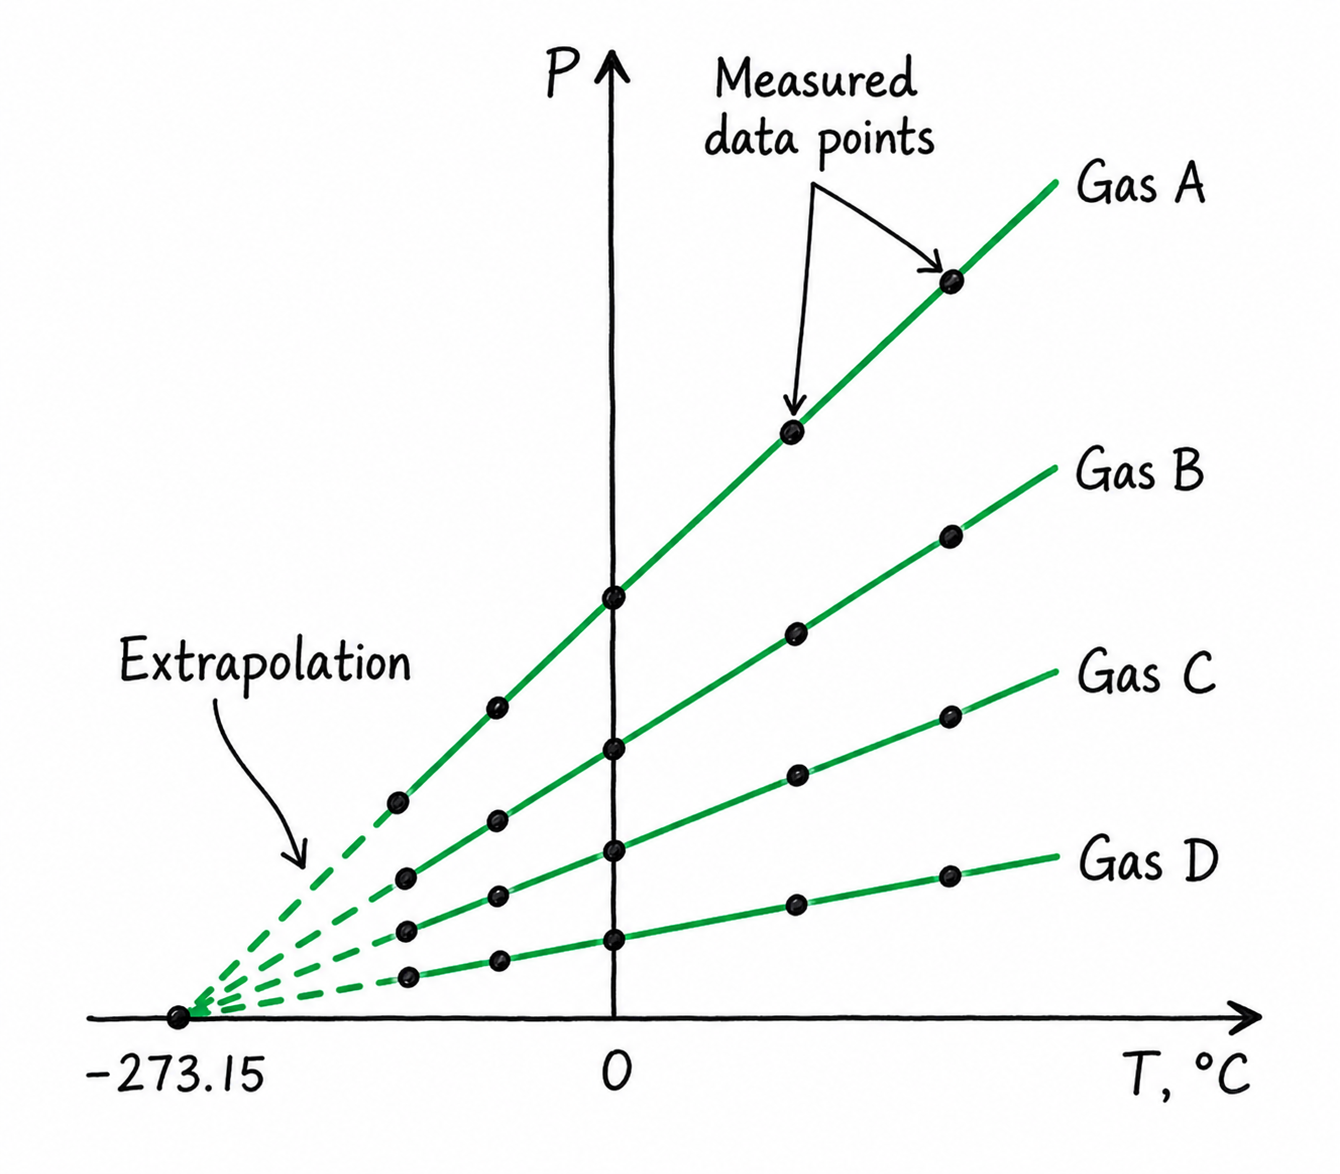
\includegraphics[width=0.6\textwidth]{../2. Figures/Figure : 4.png}}
    \label{fig:myimage}
\end{figure}



\mysubsection{}{Temperature Conversion Relations}

The Kelvin and Celsius scales are related by

\begin{equation*}
    T(K) = T(^\circ\mathrm{C}) + 273.15
\end{equation*}

The Rankine and Fahrenheit scales are related by

\begin{equation*}
    T(R) = T(^\circ\mathrm{F}) + 459.67
\end{equation*}

The Rankine and Kelvin scales are related by

\begin{equation*}
    T(R) = 1.8T(K)
\end{equation*}

The Fahrenheit and Celsius scales are related by

\begin{equation*}
    T(^\circ\mathrm{F}) = 1.8T(^\circ\mathrm{C}) + 32
\end{equation*}

For ordinary engineering calculations, the constants $273.15$ and $459.67$ are sometimes rounded to $273$ and $460$, respectively.

\mysubsection{}{Temperature Differences}

The magnitude of one kelvin is identical to the magnitude of one degree Celsius.

Therefore,

\begin{equation*}
    \Delta T(K) = \Delta T(^\circ\mathrm{C})
\end{equation*}

Similarly, the magnitude of one rankine is identical to the magnitude of one degree Fahrenheit.

Therefore,

\begin{equation*}
    \Delta T(R) = \Delta T(^\circ\mathrm{F})
\end{equation*}

The relationship between the magnitudes of the units is

\begin{equation*}
    1\ K = 1^\circ\mathrm{C} = 1.8\ R = 1.8^\circ\mathrm{F}
\end{equation*}

Thus, increasing a temperature by $10^\circ\mathrm{C}$ is equivalent to increasing it by $10\ K$.

\textbf{\\ Temperature in Thermodynamic Relations}

When a thermodynamic relation contains a \textbf{temperature difference}, either K or $^\circ\mathrm{C}$ may be used because their interval magnitudes are identical.

However, when a relation contains the \textbf{temperature itself}, the absolute temperature scale must be used. In the SI system, this means using K rather than $^\circ\mathrm{C}$.

When in doubt, Kelvin is the safe choice for thermodynamic equations involving absolute temperature.

\newpage
















\mysection{1.9}{Pressure}{1.9}

\mysubsection{}{Definition of Pressure}

Pressure is defined as the \textbf{normal force exerted by a fluid per unit area}.

\begin{equation*}
    P = \frac{F_n}{A}
\end{equation*}

where $F_n$ is the normal force acting on the surface and $A$ is the surface area.

Pressure is a \textbf{scalar quantity}. In fluids, pressure acts normal to a surface.

The SI unit of pressure is the pascal:

\begin{equation*}
    1\ \mathrm{Pa} = 1\ \mathrm{N/m^2}
\end{equation*}

The pascal is small for most engineering applications, so larger pressure units are commonly used.

\textbf{\\ Common Pressure Units}

\begin{center}
    \begin{tabular}{|c|c|}
        \hline
        \textbf{Unit} & \textbf{Equivalent} \\
        \hline
        $1\ \mathrm{kPa}$ & $10^3\ \mathrm{Pa}$ \\
        \hline
        $1\ \mathrm{MPa}$ & $10^6\ \mathrm{Pa}$ \\
        \hline
        $1\ \mathrm{bar}$ & $10^5\ \mathrm{Pa}$ \\
        \hline
        $1\ \mathrm{atm}$ & $101325\ \mathrm{Pa}$ \\
        \hline
        $1\ \mathrm{kgf/cm^2}$ & $9.807\times10^4\ \mathrm{Pa}$ \\
        \hline
        $1\ \mathrm{psi}$ & $1\ \mathrm{lbf/in^2}$ \\
        \hline
    \end{tabular}
\end{center}

Other useful conversions are

\begin{equation*}
    1\ \mathrm{bar} = 100\ \mathrm{kPa} = 0.1\ \mathrm{MPa}
\end{equation*}

\begin{equation*}
    1\ \mathrm{atm} = 101.325\ \mathrm{kPa}
    = 1.01325\ \mathrm{bar}
\end{equation*}

\begin{equation*}
    1\ \mathrm{atm} = 14.696\ \mathrm{psi}
\end{equation*}

\begin{equation*}
    1\ \mathrm{kgf/cm^2}
    = 0.9807\ \mathrm{bar}
    = 0.9679\ \mathrm{atm}
    = 14.223\ \mathrm{psi}
\end{equation*}

\textbf{\\ Pressure on Solid Surfaces}

Pressure can also be used for the normal stress exerted on a solid surface.

For example, if a person's weight is $150\ \mathrm{lbf}$ and the total area of the feet is $50\ \mathrm{in^2}$,

\begin{equation*}
    P = \frac{150}{50}
    = 3\ \mathrm{psi}
\end{equation*}

Reducing the contact area increases the pressure for the same force.

This explains why:
\begin{itemize}
    \item snowshoes prevent a person from sinking deeply into snow, and
    \item a sharp knife cuts more easily than a blunt knife.
\end{itemize}

\mysubsection{}{Absolute, Gage, and Vacuum Pressure}

The pressure at a given location measured relative to absolute vacuum is called \textbf{absolute pressure}.

Absolute vacuum corresponds to zero absolute pressure.

Most pressure-measuring devices are calibrated to read zero at the local atmospheric pressure. Therefore, they indicate the difference between the absolute pressure and the atmospheric pressure.

This difference is called \textbf{gage pressure}.

\textbf{\\ Absolute Pressure}

Absolute pressure is measured relative to absolute vacuum.

\begin{equation*}
    P_{\mathrm{abs}} = 0
\end{equation*}

at absolute vacuum.

\textbf{\\ Gage Pressure}

Gage pressure is the pressure measured relative to the local atmospheric pressure.

\begin{equation*}
    P_{\mathrm{gage}} = P_{\mathrm{abs}} - P_{\mathrm{atm}}
\end{equation*}

Gage pressure may be positive or negative.

\textbf{\\ Vacuum Pressure}

When the absolute pressure is below atmospheric pressure, the difference is called \textbf{vacuum pressure}.

\begin{equation*}
    P_{\mathrm{vac}} = P_{\mathrm{atm}} - P_{\mathrm{abs}}
\end{equation*}

\textbf{\\ Pressure Relationships}

\begin{equation*}
    P_{\mathrm{abs}} = P_{\mathrm{atm}} + P_{\mathrm{gage}}
\end{equation*}

\begin{equation*}
    P_{\mathrm{abs}} = P_{\mathrm{atm}} - P_{\mathrm{vac}}
\end{equation*}

\begin{center}
    \begin{tabular}{|c|c|c|}
        \hline
        \textbf{Pressure} & \textbf{Reference} & \textbf{Typical Meaning} \\
        \hline
        Absolute & Absolute vacuum & Actual pressure \\
        \hline
        Gage & Atmospheric pressure & Pressure above or below atmosphere \\
        \hline
        Vacuum & Atmospheric pressure & Amount by which pressure is below atmosphere \\
        \hline
    \end{tabular}
\end{center}

In thermodynamic relations and tables, pressure is generally taken to mean \textbf{absolute pressure} unless otherwise specified.

The suffixes ``a'' and ``g'' may be attached to pressure units:

\begin{center}
    \begin{tabular}{|c|c|}
        \hline
        \textbf{Notation} & \textbf{Meaning} \\
        \hline
        psia & Pounds per square inch absolute \\
        \hline
        psig & Pounds per square inch gage \\
        \hline
    \end{tabular}
\end{center}

\textbf{\\ Example : }

A vacuum gage connected to a chamber reads $5.8\ \mathrm{psi}$ at a location where the atmospheric pressure is $14.5\ \mathrm{psi}$.

The absolute pressure is

\begin{equation*}
    P_{\mathrm{abs}}
    = P_{\mathrm{atm}} - P_{\mathrm{vac}}
    = 14.5 - 5.8
    = 8.7\ \mathrm{psi}
\end{equation*}

Thus, the chamber pressure is $8.7\ \mathrm{psia}$.

\mysubsection{}{Variation of Pressure with Depth}

In a fluid at rest, pressure does not change in the horizontal direction.

Therefore, all points lying on the same horizontal plane within the same continuous fluid have the same pressure.

Pressure does, however, vary in the vertical direction because of gravity.

\textbf{\\ Pressure Increase with Depth}

Pressure increases with depth because a deeper fluid layer supports a greater amount of fluid above it.

For a constant-density fluid, the pressure difference between two points is

\begin{equation*}
    \Delta P = P_2-P_1 = -\rho g\Delta z
\end{equation*}

where $\Delta z=z_2-z_1$.

Since pressure increases as elevation decreases, a convenient form is

\begin{equation*}
    P_{\mathrm{below}}
    = P_{\mathrm{above}} + \rho g|\Delta z|
\end{equation*}

Using specific weight,

\begin{equation*}
    P_{\mathrm{below}}
    = P_{\mathrm{above}} + \gamma_s|\Delta z|
\end{equation*}

where

\begin{equation*}
    \gamma_s = \rho g
\end{equation*}

\textbf{\\ Pressure Head}

For a given fluid, the vertical distance corresponding to a pressure difference is called the \textbf{pressure head}.

Pressure therefore depends on:
\begin{itemize}
    \item the vertical distance between the points,
    \item the density of the fluid, and
    \item the gravitational acceleration.
\end{itemize}



\textbf{\\ Pressure Variation in Gases}

For gases, the density is usually very low. Therefore, over small to moderate elevation changes, the variation of pressure with height is negligible.

Consequently, the pressure inside a gas-filled tank or within a room can often be approximated as uniform.

For fluids whose density varies significantly with elevation,

\begin{equation*}
    \frac{dP}{dz} = -\rho g
\end{equation*}

The pressure difference between two points is then

\begin{equation*}
    \Delta P
    = P_2-P_1
    = -\int_1^2 \rho g\,dz
\end{equation*}

For constant density and constant gravitational acceleration, this expression reduces to the hydrostatic relation.

\mysubsection{}{Hydrostatic Pressure and Container Shape}

For a fluid at rest, the pressure is independent of the shape or cross-sectional geometry of the container.

It changes only with vertical position.

Therefore, all points on the same horizontal plane in the same interconnected fluid have the same pressure.

\begin{equation*}
    P_A=P_B=P_C=P_D=P_E=P_F=P_G
\end{equation*}

provided that the points are at the same elevation and are interconnected through the same continuous static fluid.

However, points at the same depth do not necessarily have the same pressure when they belong to different fluids or are not interconnected through the same fluid.

The pressure force exerted by a fluid is always \textbf{normal to the surface} on which it acts.

\begin{figure}[H] % h = here, t = top, b = bottom, p = page of floats
    \centering
    \fbox{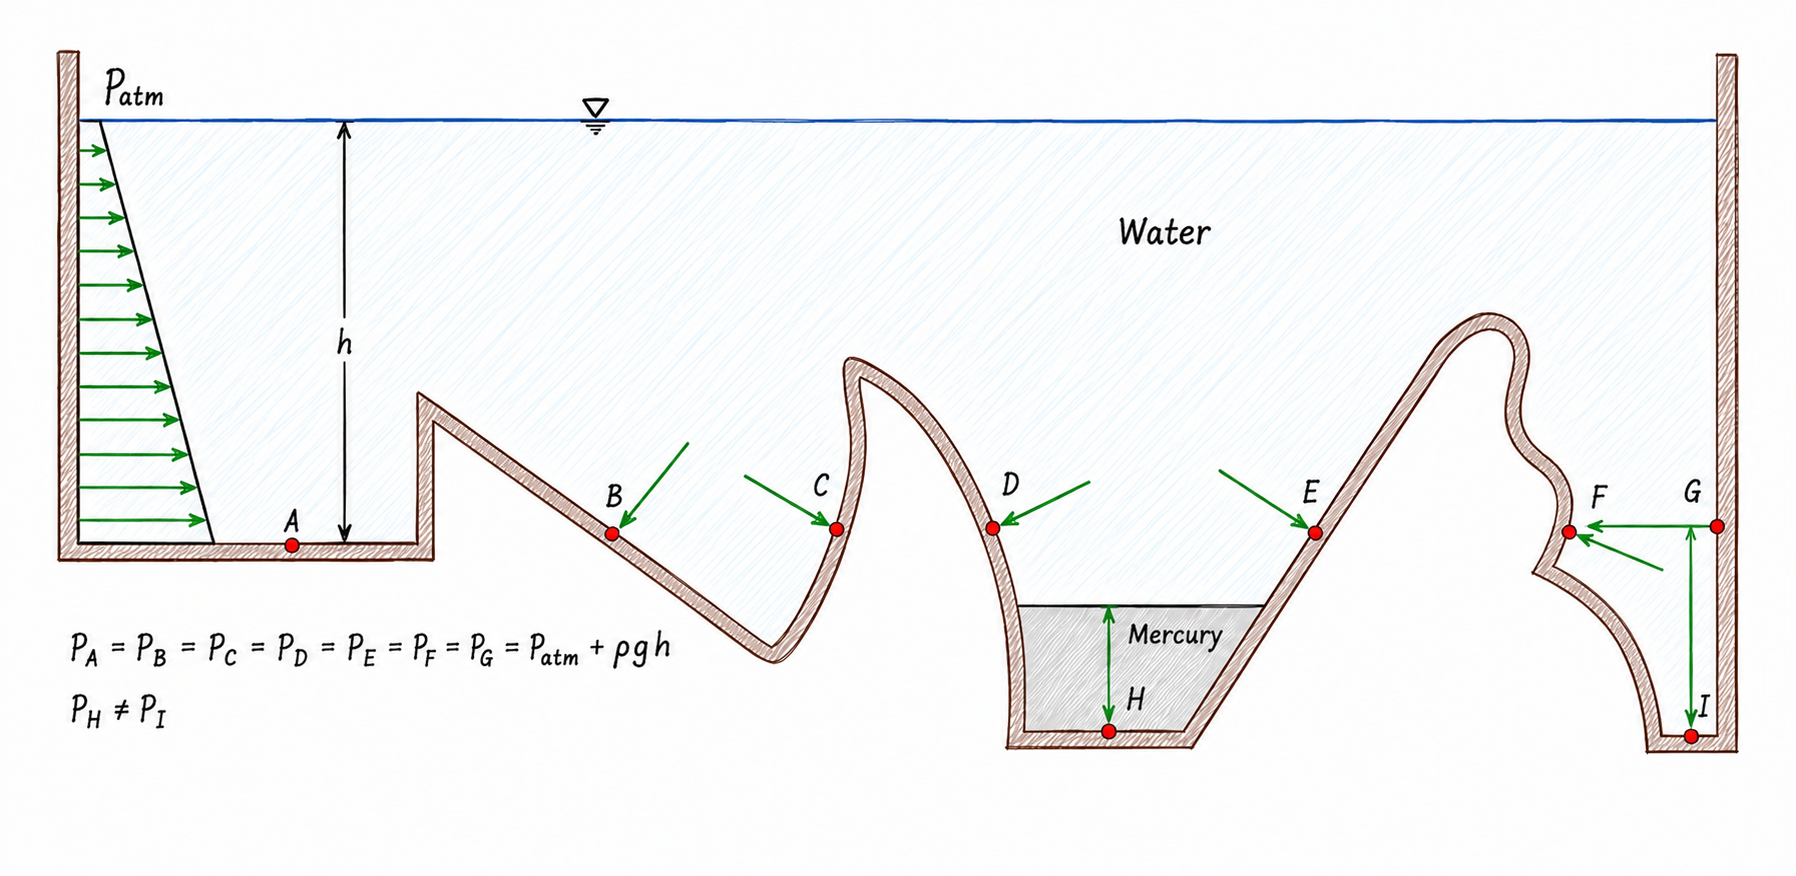
\includegraphics[width=0.8\textwidth]{../2. Figures/Figure : 5.png}}
    \label{fig:myimage}
\end{figure}

\mysubsection{}{Pascal's Law}

A consequence of pressure being uniform in the horizontal direction is that when pressure is applied to a confined fluid, the pressure increases by the same amount throughout the fluid.

This is known as \textbf{Pascal's law}.

Pascal's law forms the operating principle of hydraulic devices such as hydraulic lifts, hydraulic jacks, and hydraulic brakes.

For two connected pistons at the same level,

\begin{equation*}
    P_1=P_2
\end{equation*}

Since

\begin{equation*}
    P_1=\frac{F_1}{A_1}
\end{equation*}

and

\begin{equation*}
    P_2=\frac{F_2}{A_2}
\end{equation*}

we obtain

\begin{equation*}
    \frac{F_1}{A_1}
    =
    \frac{F_2}{A_2}
\end{equation*}

Therefore,

\begin{equation*}
    \frac{F_2}{F_1}
    =
    \frac{A_2}{A_1}
\end{equation*}

The ratio

\begin{equation*}
    \frac{A_2}{A_1}
\end{equation*}

is called the \textbf{ideal mechanical advantage} of a hydraulic lift.

Thus, a larger piston can produce a larger output force for a relatively small input force.

\textbf{\\ Example : }

For a hydraulic jack with

\begin{equation*}
    \frac{A_2}{A_1}=100
\end{equation*}

the ideal mechanical advantage is $100$.

Therefore,

\begin{equation*}
    F_2=100F_1
\end{equation*}

A person can therefore lift a much larger load by applying a relatively small force to the smaller piston.

\newpage

















\mysection{1.10}{Pressure Measurement Devices}{1.10}

\mysubsection{}{The Barometer}

A \textbf{barometer} is a device used to measure atmospheric pressure. Therefore, atmospheric pressure is also called \textbf{barometric pressure}.

The basic barometer consists of a mercury-filled tube inverted into a container of mercury that is open to the atmosphere. The space above the mercury column contains only a very small amount of mercury vapor and can be treated as a vacuum.

At equilibrium, the atmospheric pressure supports the mercury column. A force balance gives

\begin{equation*}
    P_{\mathrm{atm}} = \rho g h
\end{equation*}

where:
\begin{itemize}
    \item $P_{\mathrm{atm}}$ = atmospheric pressure,
    \item $\rho$ = density of mercury,
    \item $g$ = local gravitational acceleration,
    \item $h$ = height of the mercury column.
\end{itemize}

The height of the mercury column is independent of the length and cross-sectional area of the tube, provided the tube is sufficiently large to make capillary effects negligible.

\begin{figure}[H] % h = here, t = top, b = bottom, p = page of floats
    \centering
    \fbox{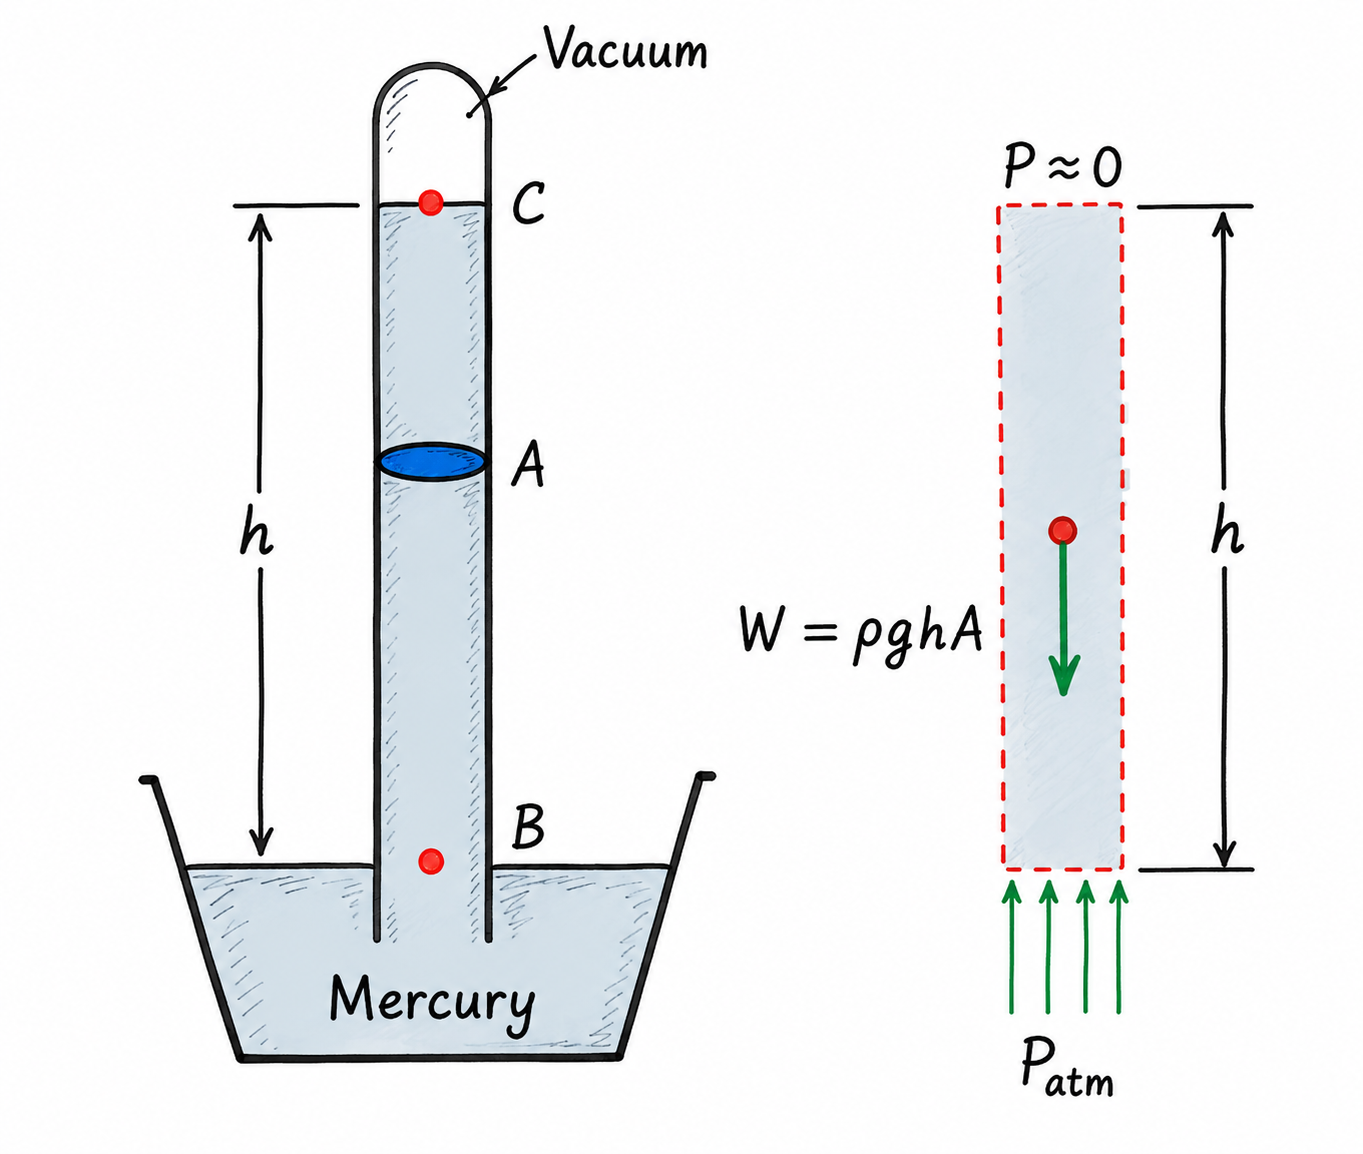
\includegraphics[width=0.6\textwidth]{../2. Figures/Figure : 6.png}}
    \label{fig:myimage}
\end{figure}


\textbf{\\ Standard Atmospheric Pressure}

A standard atmosphere is defined as the pressure produced by a mercury column $760\ \mathrm{mm}$ high at $0^\circ\mathrm{C}$ under standard gravitational acceleration.

\begin{equation*}
    1\ \mathrm{atm} = 760\ \mathrm{mmHg}
\end{equation*}

Since millimeters of mercury are also called torr,

\begin{equation*}
    1\ \mathrm{atm} = 760\ \mathrm{torr}
\end{equation*}

and

\begin{equation*}
    1\ \mathrm{torr} \approx 133.3\ \mathrm{Pa}
\end{equation*}

If water were used instead of mercury, a water column of approximately $10.3\ \mathrm{m}$ would be required to produce standard atmospheric pressure.

\textbf{\\ Variation of Atmospheric Pressure with Elevation}

Atmospheric pressure decreases as elevation increases because the weight of the air above a location decreases.

The atmospheric pressure is approximately:
\begin{center}
    \begin{tabular}{|c|c|}
        \hline
        \textbf{Elevation} & \textbf{Atmospheric Pressure} \\
        \hline
        Sea level & $101.325\ \mathrm{kPa}$ \\
        \hline
        $1000\ \mathrm{m}$ & $89.88\ \mathrm{kPa}$ \\
        \hline
        $2000\ \mathrm{m}$ & $79.50\ \mathrm{kPa}$ \\
        \hline
        $5000\ \mathrm{m}$ & $54.05\ \mathrm{kPa}$ \\
        \hline
        $10000\ \mathrm{m}$ & $26.5\ \mathrm{kPa}$ \\
        \hline
        $20000\ \mathrm{m}$ & $5.53\ \mathrm{kPa}$ \\
        \hline
    \end{tabular}
\end{center}

Atmospheric pressure at a location is determined by the weight of the air above that location per unit area. It therefore changes with both elevation and weather conditions.

The decrease in atmospheric pressure with elevation has practical effects:
\begin{itemize}
    \item water boils at a lower temperature at high elevations,
    \item less oxygen is available per unit volume of air,
    \item internal-combustion engines produce less power unless compensated, and
    \item aircraft experience changes in lift and drag because of the lower air density.
\end{itemize}

\textbf{\\ Example : }

A barometer reads $740\ \mathrm{mmHg}$ at a location where

\begin{equation*}
    g = 9.805\ \mathrm{m/s^2}
\end{equation*}

and the density of mercury at the specified temperature is

\begin{equation*}
    \rho_{\mathrm{Hg}} = 13570\ \mathrm{kg/m^3}
\end{equation*}

The atmospheric pressure is

\begin{equation*}
    P_{\mathrm{atm}} = \rho gh
\end{equation*}

\begin{equation*}
    P_{\mathrm{atm}}
    =
    (13570)(9.805)(0.740)
    =
    98.5\ \mathrm{kPa}
\end{equation*}

Thus, the barometer reading can be converted directly into atmospheric pressure using the hydrostatic relation.

\mysubsection{}{The Manometer}

A \textbf{manometer} is a pressure-measuring device that uses a liquid column to determine a pressure difference.

Manometers are commonly used to measure \textbf{small and moderate pressure differences}.

A simple manometer consists of a glass or plastic U-tube containing one or more fluids such as:
\begin{itemize}
    \item mercury,
    \item water,
    \item alcohol, or
    \item oil.
\end{itemize}

Heavy fluids such as mercury are useful when large pressure differences must be measured because a smaller column height can then produce the required pressure difference.

The basic principle follows from hydrostatics:

\begin{equation*}
    \Delta P = \rho gh
\end{equation*}

Pressure increases when moving downward through a fluid and decreases when moving upward.

For a manometer open to the atmosphere,

\begin{equation*}
    P_2 = P_{\mathrm{atm}} + \rho gh
\end{equation*}

where $h$ is the difference in fluid-column elevation.

The cross-sectional area of the tube does not affect the pressure difference produced by a given height difference. However, the tube diameter should be sufficiently large to minimize capillary effects.

\textbf{\\ Important Rules for Manometer Analysis}

When moving through a manometer:
\begin{center}
    \begin{tabular}{|c|c|}
        \hline
        \textbf{Movement} & \textbf{Pressure change} \\
        \hline
        Downward through a fluid & Add $\rho gh$ \\
        \hline
        Upward through a fluid & Subtract $\rho gh$ \\
        \hline
        Horizontally in the same continuous fluid & No pressure change \\
        \hline
    \end{tabular}
\end{center}

Thus, the pressure at an unknown point can be found by starting from a point of known pressure and adding or subtracting the appropriate $\rho gh$ terms.



\textbf{\\ Inclined Manometer}

An \textbf{inclined manometer} uses a slanted tube to increase the displacement of the liquid column for a given pressure difference.

This increases the \textbf{resolution} and makes small pressure differences easier to measure accurately.

\mysubsection{}{Multifluid Manometers}

Some manometers contain several immiscible fluids with different densities.

The analysis is based on three rules:
\begin{enumerate}
    \item The pressure change across a fluid column of height $h$ is $\rho gh$.
    \item Pressure increases downward and decreases upward.
    \item Two points at the same elevation in the same continuous fluid at rest have the same pressure.
\end{enumerate}

For stacked fluid layers, starting from a point of known pressure and moving downward through each layer gives

\begin{equation*}
    P_{\mathrm{bottom}}
    =
    P_{\mathrm{top}}
    +
    \rho_1gh_1
    +
    \rho_2gh_2
    +
    \rho_3gh_3
\end{equation*}

If all fluids have the same density, this reduces to

\begin{equation*}
    P_{\mathrm{bottom}}
    =
    P_{\mathrm{top}}
    +
    \rho g(h_1+h_2+h_3)
\end{equation*}

\textbf{\\ Differential Manometer}

A differential manometer measures the pressure difference between two specified points, often across a flow device such as a valve, heat exchanger, or other flow resistance.

For the arrangement shown in the section, the pressure difference is

\begin{equation*}
    P_1-P_2
    =
    (\rho_2-\rho_1)gh
\end{equation*}

where:
\begin{itemize}
    \item $\rho_1$ = density of the flowing fluid,
    \item $\rho_2$ = density of the manometer fluid,
    \item $h$ = differential fluid height.
\end{itemize}

For a gas flowing in the pipe, $\rho_1$ is much smaller than $\rho_2$, so

\begin{equation*}
    P_1-P_2 \approx \rho_2gh
\end{equation*}


\newpage

\begin{figure}[H] % h = here, t = top, b = bottom, p = page of floats
    \centering
    \fbox{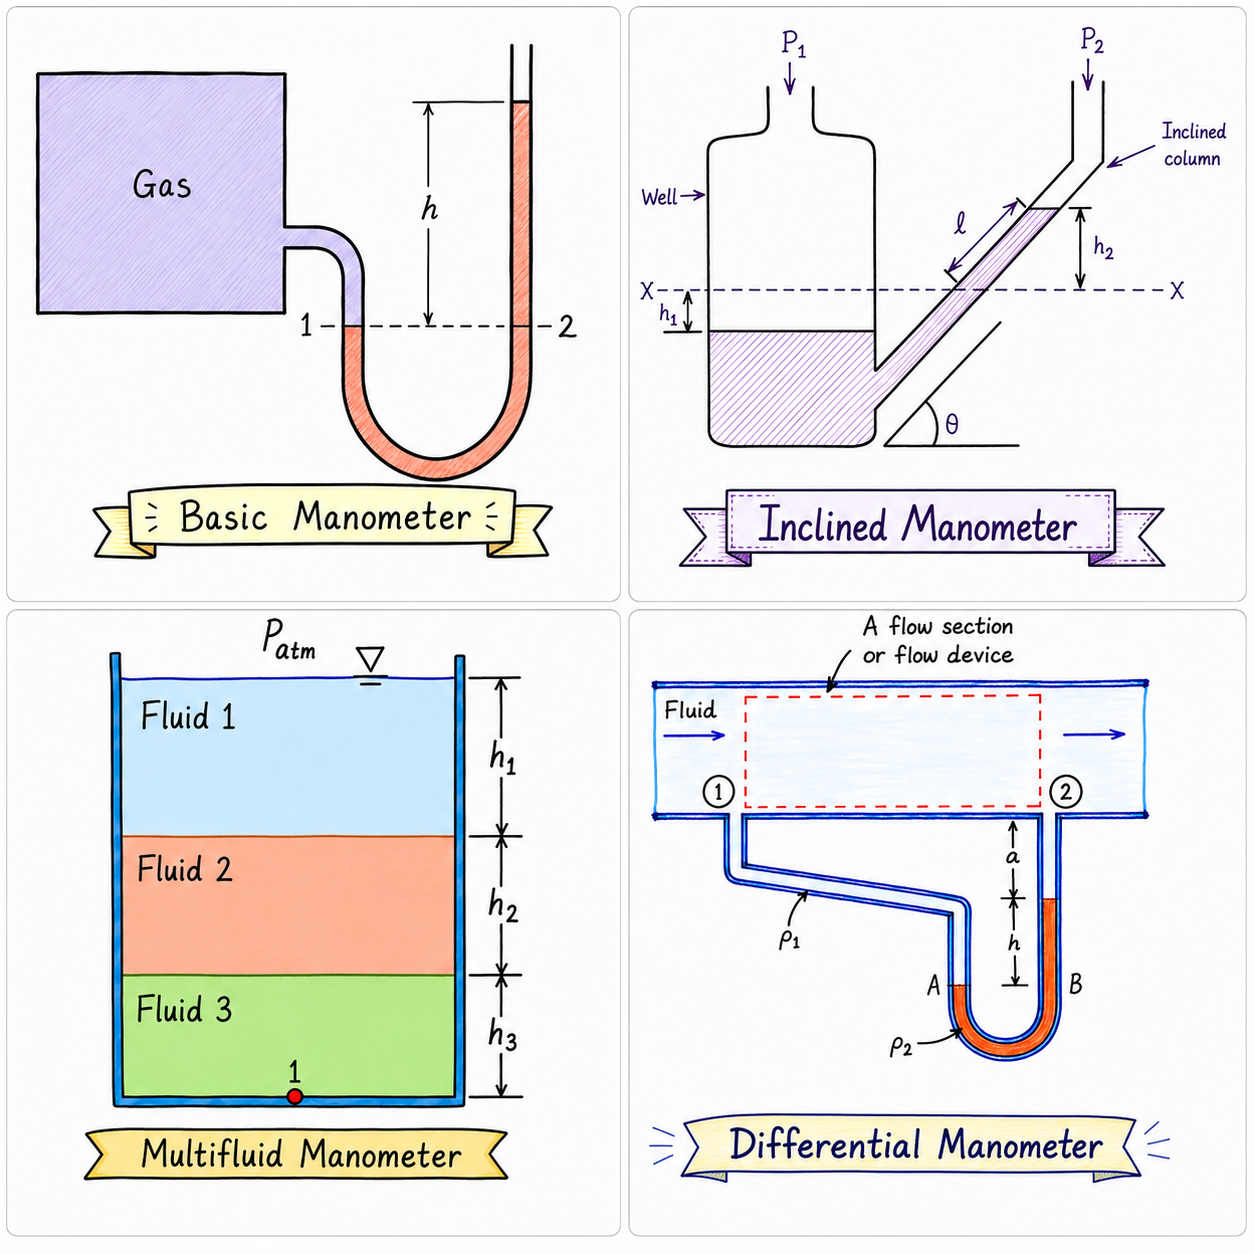
\includegraphics[width=\textwidth]{../2. Figures/Figure : 7.png}}
    \label{fig:myimage}
\end{figure}

\newpage
















\mysection{1.11}{Problem-Solving Technique}{1.11}

\mysubsection{}{Systematic Problem Solving}

Solving engineering problems, especially complicated ones, requires a \textbf{systematic approach}. A step-by-step method reduces a complicated problem to a series of simpler tasks and helps avoid common errors.

The recommended problem-solving procedure consists of seven steps.

\textbf{\\ Step 1: Problem Statement}

State the problem briefly in your own words.

The problem statement should include:
\begin{itemize}
    \item the key information given,
    \item the quantities that must be determined, and
    \item the main objective of the analysis.
\end{itemize}

This ensures that the physical problem and its objectives are understood before beginning the solution.

\textbf{\\ Step 2: Schematic}

Draw a realistic sketch of the physical system and include the relevant information directly on the figure.

The schematic should show the important features of the system and may include:
\begin{itemize}
    \item dimensions,
    \item known properties,
    \item unknown quantities,
    \item energy interactions,
    \item mass interactions, and
    \item properties that remain constant during the process.
\end{itemize}

The sketch does not need to be elaborate, but it should represent the physical system clearly.

\textbf{\\ Step 3: Assumptions and Approximations}

State the assumptions and approximations used to simplify the problem.

Questionable assumptions should be justified, and reasonable values may be assumed for missing information when necessary.

For example, if no atmospheric pressure is specified, $1\ \mathrm{atm}$ may be assumed in some situations. However, the effect of elevation should be considered when appropriate because atmospheric pressure decreases with elevation.

\textbf{\\ Step 4: Physical Laws}

Apply all relevant physical laws and principles to the system.

Examples include:
\begin{itemize}
    \item conservation of mass,
    \item conservation of energy, and
    \item other fundamental physical relations.
\end{itemize}

The region or system to which each physical law is applied must first be identified clearly.

For example, the increase in velocity of water flowing through a nozzle can be analyzed by applying conservation of mass between the inlet and outlet.

\textbf{\\ Step 5: Properties}

Determine the unknown properties at known states that are required for the solution.

These properties may be obtained from:
\begin{itemize}
    \item property relations, or
    \item thermodynamic property tables.
\end{itemize}

Properties should be listed separately, and their source should be identified when appropriate.

\textbf{\\ Step 6: Calculations}

Substitute the known quantities into the simplified physical relations and calculate the required unknowns.

Special attention should be given to:
\begin{itemize}
    \item units,
    \item unit cancellations, and
    \item appropriate significant digits.
\end{itemize}

A dimensional quantity without a unit is meaningless. Intermediate calculations should retain sufficient digits, while the final result should be reported with an appropriate number of significant digits.

\textbf{\\ Step 7: Reasoning, Verification, and Discussion}

The final results should be checked to determine whether they are physically reasonable and intuitive.

The analysis should include:
\begin{itemize}
    \item verification of questionable assumptions,
    \item repetition of calculations that produce unreasonable results,
    \item interpretation of the significance of the results,
    \item conclusions and recommendations where appropriate, and
    \item limitations under which the results are valid.
\end{itemize}

The results should not be applied to situations in which the underlying assumptions are invalid.

\mysubsection{}{Importance of Organization}

Engineering solutions are also a form of communication. Therefore, \textbf{neatness, organization, completeness, and visual clarity} are important.

A well-organized solution helps reveal errors and inconsistencies. Skipping steps merely to save time can lead to additional errors and wasted effort.

Not every problem requires every step to be written explicitly. Some steps may be unnecessary for simple problems. Nevertheless, a logical and orderly approach is strongly recommended.

Many difficulties in solving engineering problems arise not from lack of knowledge, but from a lack of organization.

\newpage


\begin{center}
\vspace{15pt}
{\headingfont\Huge Significant Digits}
\par
\vspace{4pt}
\hrule

\end{center}


Engineering calculations are meaningful only to the precision of the measured
data. Reporting more digits than justified gives a \textbf{false impression of
accuracy}. Therefore, the final answer should never contain more significant
digits than the least precise quantity used in the calculation. 

%------------------------------------------------

\vspace{15pt}
{\headingfont\large Definition}
\par
\vspace{4pt}
\hrule
\vspace{10pt}

\textbf{Significant digits} are the digits in a measured quantity that carry
meaning regarding its precision.

For example,

\[
3.75~\text{L}
\]

contains \textbf{three significant digits} because the digits \(3\), \(7\), and
\(5\) are all known to be meaningful.

%------------------------------------------------

\vspace{15pt}
{\headingfont\large Why Significant Digits matter}
\par
\vspace{4pt}
\hrule
\vspace{10pt}
Suppose a container has

\[
V=3.75~\text{L},
\qquad
\rho=0.845~\text{kg/L}.
\]

A calculator gives

\[
m=V\rho
=3.75\times0.845
=3.16875~\text{kg}.
\]

Although mathematically correct, writing

\[
3.16875~\text{kg}
\]

is misleading because both the volume and density are known only to
\textbf{three significant digits}. Hence the result cannot be more accurate
than three significant digits.

Therefore,

\[
\boxed{m=3.17~\text{kg}}
\]

is the correct engineering answer. 

%------------------------------------------------
\vspace{15pt}
{\headingfont\large Why can't we keep more digits}
\par
\vspace{4pt}
\hrule
\vspace{10pt}
The value

\[
3.75~\text{L}
\]

does not mean the volume is exactly \(3.750000\) L.

Instead, it means the measurement is accurate only to the hundredths place.

Possible actual values include

\[
3.746,\;
3.750,\;
3.753,\;
\ldots
\]

because all round to

\[
3.75.
\]

Similarly,

\[
0.845~\text{kg/L}
\]

does not imply infinite precision.

Thus multiplying these measurements cannot produce a result accurate to six
significant digits. 

%------------------------------------------------

\vspace{15pt}
{\headingfont\large Engineering Practice}
\par
\vspace{4pt}
\hrule
\vspace{10pt}

When performing calculations,

\begin{itemize}
\item keep all calculator digits during intermediate steps,
\item round only the final answer,
\item report only the number of significant digits justified by the given data.
\end{itemize}

%------------------------------------------------

\vspace{15pt}
{\headingfont\large Measurement Uncertainity}
\par
\vspace{4pt}
\hrule
\vspace{10pt}
Every experimentally measured quantity contains some uncertainty.

For example,

\begin{itemize}
\item if density has an uncertainty of \(2\%\),
\item then any mass calculated using that density also has approximately
\(2\%\) uncertainty.
\end{itemize}

Thus extremely precise numerical answers are generally meaningless because
the measurements themselves are not exact. 

%------------------------------------------------

\vspace{15pt}
{\headingfont\large Engineering Approximations}
\par
\vspace{4pt}
\hrule
\vspace{10pt}

Engineers often intentionally introduce small approximations to simplify
calculations.

Example:

Instead of using the exact density of water at \(75^\circ\mathrm{C}\),

\[
\rho=975~\text{kg/m}^3,
\]

it is common to use

\[
\rho=1000~\text{kg/m}^3.
\]

This introduces only about a \(2.5\%\) error, which is acceptable in many
engineering calculations because other experimental uncertainties are usually
of comparable magnitude. Therefore, rounding final answers to a reasonable
number of significant digits is both acceptable and recommended. 

%------------------------------------------------
\newpage

\vspace{15pt}
{\headingfont\large Practical Rules}
\par
\vspace{4pt}
\hrule
\vspace{10pt}

\begin{enumerate}
\item Never report more significant digits than justified by the least precise input.
\item Retain full calculator precision during intermediate calculations.
\item Round only the final answer.
\item More digits do \textbf{not} imply greater accuracy.
\item Experimental uncertainty limits the precision of every engineering calculation.
\end{enumerate}


\textbf{Question:}

In the context of significant digits, if I say \(3.75\), can the actual value range from \(3.746\) to \(3.755\), basically \(\pm\) half of a thousandth?

\bigskip

\textbf{Answer:}

Not exactly. Since \(3.75\) is rounded to two decimal places (or three significant figures), the last retained digit is in the hundredths place, so the maximum rounding error is half of one hundredth:

\[
\pm \frac{0.01}{2} = \pm 0.005.
\]

Thus, the actual value lies within

\[
3.75 \pm 0.005.
\]

This corresponds to the interval

\[
3.745 \le x < 3.755.
\]

The lower bound is inclusive because \(3.745\) rounds to \(3.75\), while the upper bound is exclusive because \(3.755\) rounds to \(3.76\).

Therefore, the correct range is

\[
\boxed{3.745 \le x < 3.755.}
\]

The general rule is that the uncertainty associated with a rounded number is equal to \textbf{half the value of the least significant digit}.





\end{document}